\documentclass[12pt, a4paper]{article}
\usepackage{multirow}
% utilizzato per inserire foto
\usepackage[draft]{graphicx}
\usepackage{longtable}
% Utilizzato per convertire alcuni testi di default in italiano
\usepackage[italian]{babel}
% permette agli hypertext di essere cliccabili
\usepackage{hyperref}
\hypersetup{
    colorlinks,
    citecolor=black,
    filecolor=black,
    linkcolor=black,
    urlcolor=magenta
}
\usepackage[table,xcdraw]{xcolor}
% FONT
\usepackage{newtxtext}
\usepackage[margin=3cm]{geometry}

% interlinea
\usepackage{setspace}
\renewcommand{\baselinestretch}{1.5} 

\newcommand{\meskip}{\medskip \\}
\newcommand{\bskip}{\bigskip \\}

\usepackage{enumitem}

% ############ JUSTIFY ############
\tolerance=1
\emergencystretch=\maxdimen
\hyphenpenalty=10000
\hbadness=10000
% #################################

\title{
    
\includegraphics[width=.8\textwidth]{images/LOGO.png}\\
    \textbf{Business Plan}
}
\date{}
\author{
    Lorenzo Sequino - N86004367 \\
    Filippo Minieri - N86004348 \\
    Simone Ingenito - N86004063 \\
    Vincenzo Di Nardo - N86004205 \\
    Roberto Ingenito - N86004077
}

\begin{document}

\maketitle

\newpage

\tableofcontents

\newpage

\section{Descrizione dell'impresa}
La nostra startup è stata fondata con un obiettivo chiaro: offrire un'esperienza enologica eccezionale a tutti gli appassionati del vino.
Siamo fermamente convinti che il vino non sia solo una bevanda, ma un'arte che merita di essere scoperta e apprezzata appieno.\meskip
Attraverso la nostra piattaforma online, abbiamo creato un ambiente virtuale in cui i nostri clienti possono immergersi nel meraviglioso mondo del vino. Offriamo loro l'opportunità di esplorare un vasto assortimento di vini provenienti da diverse regioni e cantine, consentendo loro di ampliare le loro conoscenze e scoprire nuovi gusti. Inoltre, forniamo recensioni autentiche e affidabili, garantendo ai nostri clienti una guida preziosa nella scelta del vino più adatto alle loro preferenze.\meskip
Sappiamo che la comodità è un elemento fondamentale nella vita di oggi, quindi ci assicuriamo che i nostri clienti possano godere di un'esperienza di acquisto senza problemi. Grazie al nostro sistema di ordini online, possono selezionare i loro vini preferiti e riceverli comodamente a casa propria. E per garantire che ogni bottiglia arrivi in condizioni ottimali, abbiamo stretto partnership con servizi di spedizione veloci e affidabili.\meskip
Ma c'è qualcosa che ci rende davvero speciali.
In Vinovo, mettiamo un'enfasi particolare sulla sostenibilità nel settore vinicolo.
Siamo consapevoli dell'importanza di preservare l'ambiente e lavoriamo solo con produttori che adottano pratiche ecologiche nella produzione dei loro vini.
Ci impegniamo a ridurre l'impatto ambientale, promuovendo l'uso responsabile delle risorse e incoraggiando l'agricoltura sostenibile.\meskip
In sintesi, Vinovo rappresenta molto più di una semplice piattaforma di vendita di vini. Rappresenta un'esperienza enologica completa, in cui la qualità e la sostenibilità si uniscono per offrire ai nostri clienti un viaggio indimenticabile nel mondo del vino. Vogliamo essere il punto di riferimento per tutti coloro che desiderano esplorare l'arte e il piacere di un buon bicchiere di vino, garantendo loro un accesso facile a una selezione vasta e curata.
Unisciti a noi in questo viaggio e lasciati conquistare dalla passione e dall'eccellenza che si cela dietro ogni nostra bottiglia di vino.

\subsection{Vision e mission}
\subsubsection*{Vision}
La nostra visione è quella di trasformare l'esperienza enologica in un viaggio affascinante e coinvolgente, in cui la qualità, la sostenibilità e la scoperta si fondono armoniosamente.
Vogliamo che ogni appassionato del vino possa esplorare e apprezzare i tesori enogastronomici del mondo, guidato dalla curiosità e dalla consapevolezza di fare scelte che rispettino l'ambiente.

\subsubsection*{Mission}
La nostra missione è quella di creare un legame forte tra i produttori di vini di alta qualità e i consumatori desiderosi di vivere un'esperienza enologica autentica.\\
Ci concentriamo sulla qualità dei prodotti, sulla sostenibilità delle pratiche produttive e sulla garanzia di un servizio di spedizione veloce e sicuro.\meskip
Ci adoperiamo attivamente per promuovere la sostenibilità nel settore vinicolo; vogliamo educare i consumatori sull'importanza di fare scelte sostenibili e offrire loro una selezione di vini che rispecchi questi valori.\meskip
Siamo determinati a diventare un punto di riferimento per tutti coloro che cercano\\ un'esperienza enologica autentica, basata sulla scoperta, sulla qualità e sulla sostenibilità.
Vogliamo creare una comunità in cui gli appassionati del vino possano condividere le loro esperienze, imparare dagli esperti del settore e lasciarsi ispirare da nuove tendenze e scoperte enogastronomiche.\meskip
In sintesi, la nostra visione è quella di offrire un'esperienza enologica di qualità, in cui la passione per il vino si unisce alla consapevolezza ambientale.

\subsection{Collaborazioni}
I nostri collaboratori sono una parte fondamentale del successo di Vinovo.
Collaboriamo con una rete diversificata di partner, tra cui ristoranti e locali, produttori di vini e aziende di logistica, che contribuiscono a rendere possibile la nostra missione.\meskip
I ristoranti e i locali con cui collaboriamo sono selezionati con cura per offrire ai nostri clienti un'esperienza culinaria raffinata e in sintonia con i vini di alta qualità presenti sulla nostra piattaforma.
Riconosciamo l'importanza di abbinare il vino ad una cucina di qualità, e la collaborazione con questi partner ci consente di offrire ai nostri clienti un'esperienza completa, in cui i sapori si armonizzano perfettamente.\meskip
Collaboriamo con cantine che mettono passione e impegno nella produzione di vini di alta qualità, rispettando l'ambiente.
Questa collaborazione ci consente di offrire ai nostri clienti una selezione accurata di vini unici e di raccontare le storie dietro ogni etichetta.\meskip
Le aziende di logistica con cui ci associamo sono responsabili della spedizione dei nostri vini.
Siamo consapevoli dell'importanza di garantire che ogni bottiglia arrivi in condizioni ottimali e nel minor tempo possibile.
Le aziende di logistica con cui collaboriamo condividono i nostri alti standard di affidabilità e sicurezza, garantendo che i nostri clienti possano godere dei loro vini preferiti senza preoccupazioni.\meskip
Riconosciamo il valore delle relazioni di collaborazione e crediamo nell'importanza di costruire partnership solide e durature.\meskip
Continueremo a coltivare queste partnership e a cercare nuove opportunità di collaborazione, perché crediamo che insieme possiamo offrire ai nostri clienti un viaggio indimenticabile nel mondo del vino.\newpage

\subsection{Bozza del sito web}
\begin{center}
    \frame{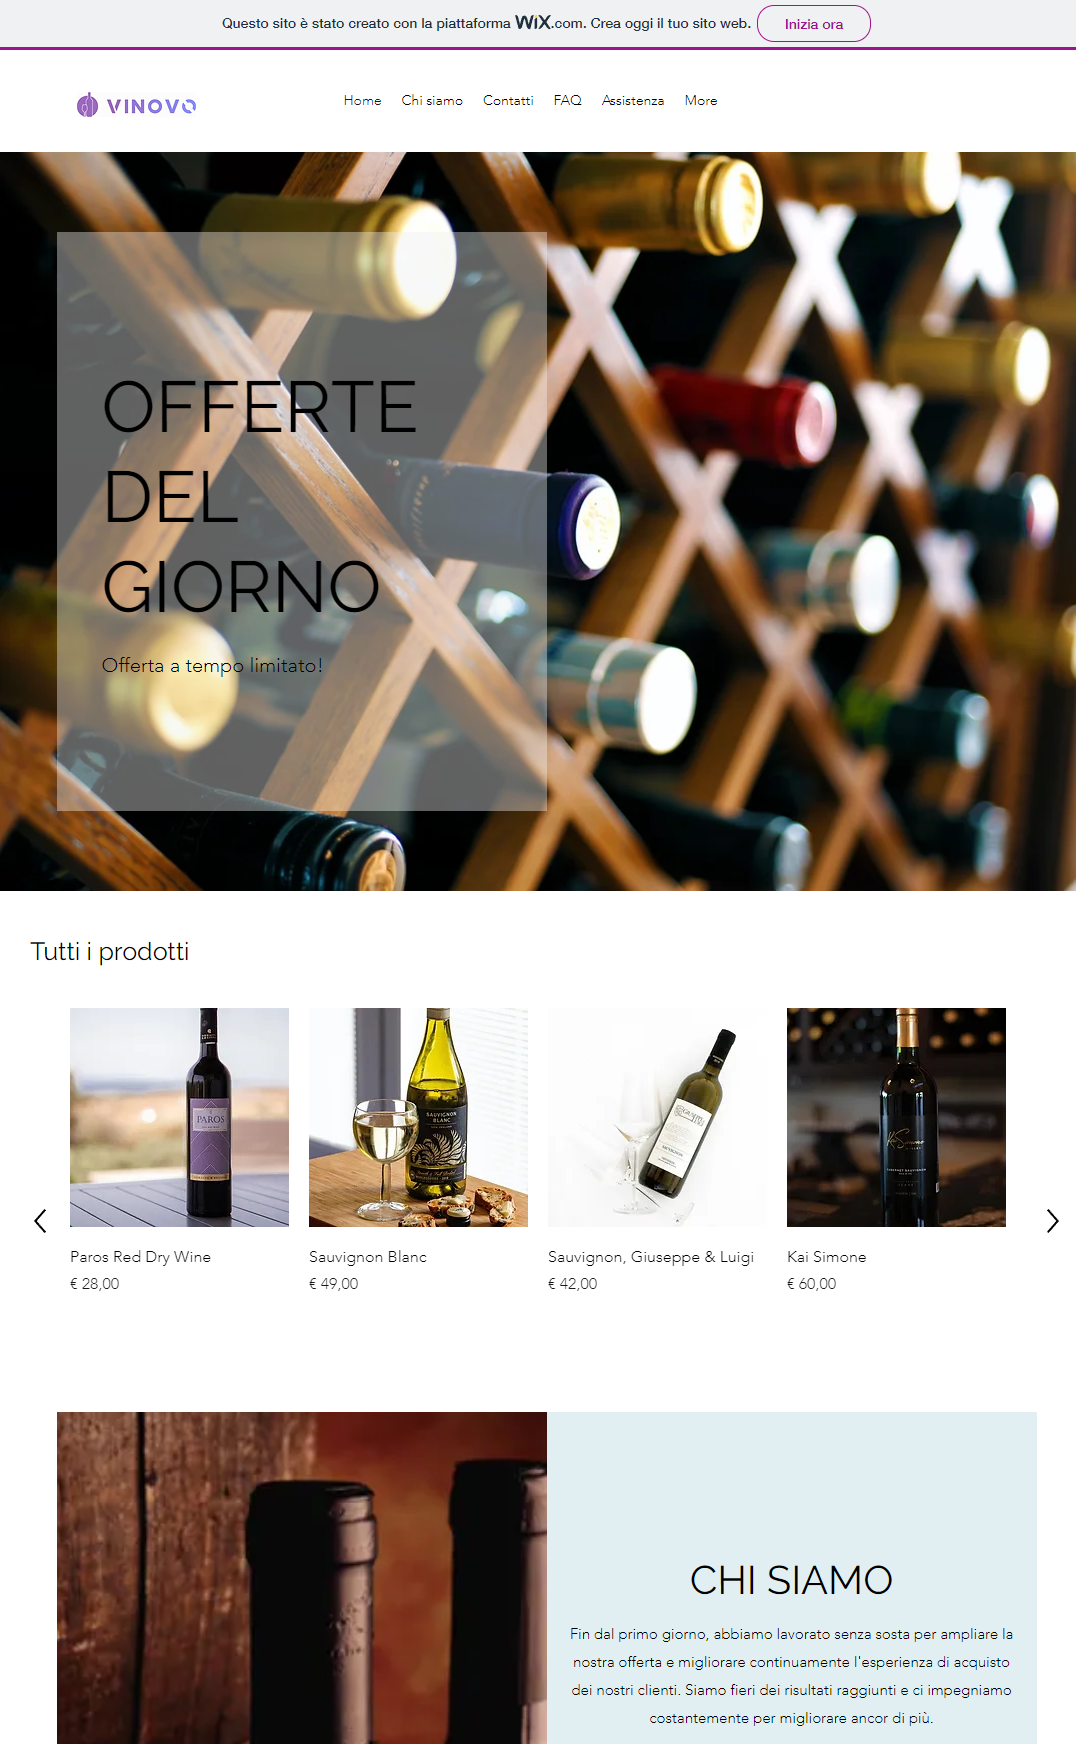
\includegraphics[width=.93\textwidth]{images/sito.png}}
\end{center}

\subsection{Fasi di produzione del vino}
La produzione del vino coinvolge diverse fasi che vanno dalla coltivazione delle viti alla vinificazione e all'invecchiamento del vino. Di seguito sono elencate le fasi dettagliate della produzione del vino:
\begin{center}
    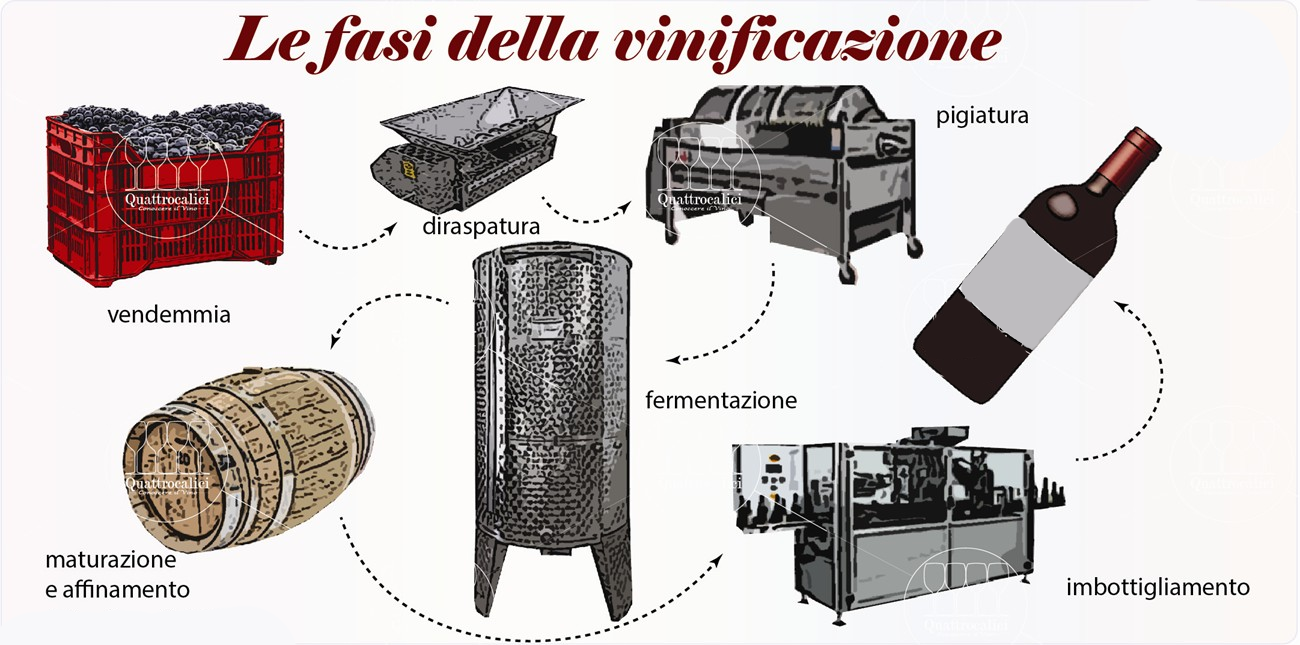
\includegraphics[width=\textwidth]{images/vinificazione-fasi-1.png}
\end{center}
\begin{itemize}
    \item \textbf{Scelta del terreno adatto}: selezione di un terreno con le caratteristiche adatte, come la composizione del suolo, il drenaggio e l'esposizione al sole.
    \item \textbf{Selezione delle varietà di uva}: identificazione delle varietà di uva più adatte al terreno e al clima della regione.
    \item \textbf{Preparazione del terreno}: lavorazione del terreno per migliorare la sua struttura e la disponibilità dei nutrienti.
    \item \textbf{Impianto dei vitigni}: piantumazione delle viti nel terreno seguendo un layout specifico.
    \item \textbf{Potatura}: taglio selettivo dei rami per controllare la crescita delle viti e favorire la qualità dell'uva.
    \item \textbf{Irrigazione}: fornitura di acqua alle piante, se necessario, per garantire una crescita sana.
    \item \textbf{Controllo delle malattie e delle infestazioni di insetti}: monitoraggio costante e adozione di misure preventive per proteggere le viti da malattie e parassiti.
    \item \textbf{Raccolta dell'uva}: determinazione del momento ottimale per la raccolta dell'uva in base al livello di zucchero, acidità e maturazione dei tannini. I grappoli maturi vengono raccolti manualmente o meccanicamente.
    \item \textbf{Selezione}: separazione delle uve danneggiate o non mature per garantire la qualità del raccolto.
    \item \textbf{Pigia-pigiatura}: schiacciamento delle uve per rompere le bucce e rilasciare il succo.
    \item \textbf{Fermentazione}: trasformazione del succo d'uva in vino attraverso l'azione dei lieviti, che convertono gli zuccheri in alcol etilico. La fermentazione può avvenire in tini di acciaio inox o in botti di legno.
    \item \textbf{Maturazione}: il vino viene lasciato invecchiare in botti di legno o serbatoi di acciaio inox per un periodo di tempo variabile, durante il quale sviluppa caratteristiche organolettiche.
    \item \textbf{Affinamento}: in alcuni casi, il vino viene sottoposto a ulteriori processi di affinamento in bottiglia per migliorarne la complessità e la struttura.
    \item \textbf{Filtrazione}: rimozione delle particelle solide sospese attraverso filtri per rendere il vino limpido.
    \item \textbf{Chiarificazione}: utilizzo di agenti di chiarificazione per rimuovere eventuali sostanze indesiderate che possono influenzare il colore o il gusto del vino.
    \item \textbf{Stabilizzazione}: applicazione di metodi per prevenire la formazione di sedimenti o precipitazioni indesiderate nel vino.
    \item \textbf{Imbottigliamento}: trasferimento del vino nelle bottiglie e chiusura con tappi di sughero o chiusure alternative.
    \item \textbf{Etichettatura}: applicazione di etichette che riportano informazioni sul vino, come il nome del produttore, l'anno di produzione e le caratteristiche del vino.
    \item \textbf{Conservazione}: conservazione delle bottiglie di vino in condizioni controllate, come temperatura e umidità, per preservarne la qualità nel tempo.
    \item \textbf{Distribuzione}: commercializzazione e distribuzione del vino ai punti vendita, ristoranti e direttamente ai clienti.
\end{itemize}
\begin{center}
    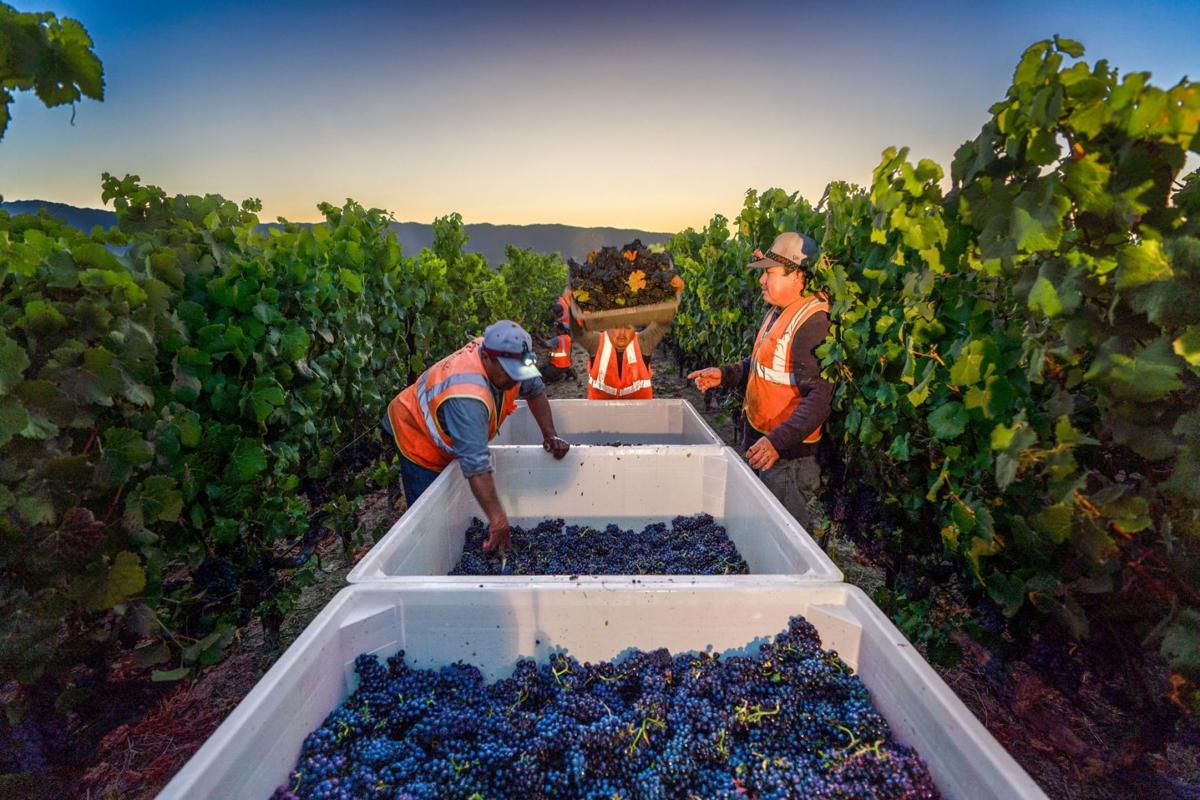
\includegraphics[width=.48\textwidth]{images/prod_vino_1.png}
    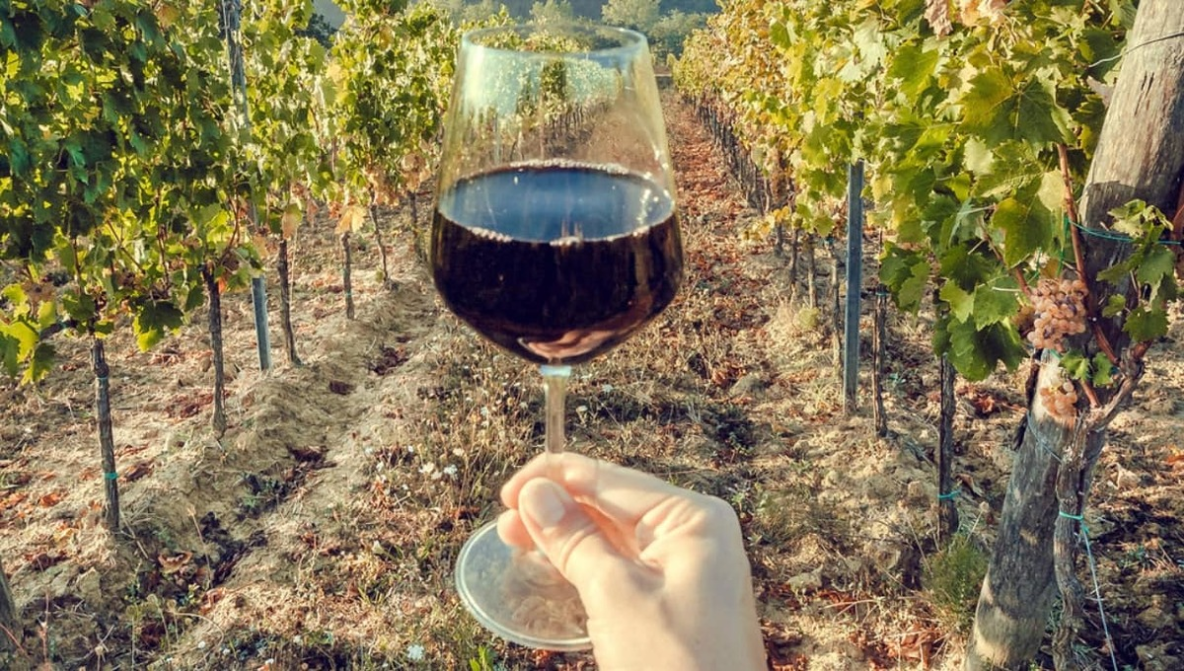
\includegraphics[width=.48\textwidth]{images/prod_vino_2.png}
\end{center}
È importante sottolineare che il processo di produzione del vino può variare a seconda delle pratiche e delle tradizioni enologiche adottate in diverse regioni e cantine vinicole

\section{Analisi di mercato}

Il settore vinicolo italiano è un pilastro dell'economia, generando un notevole fatturato annuo di 14,5 miliardi di euro. Da solo, l'export di vino vale 7,1 miliardi di euro, registrando una significativa crescita del 12,4\% nel 2021. Inoltre, la bilancia commerciale dimostra un saldo positivo di circa 6,7 miliardi di euro, confermando l'importanza strategica di questo mercato.

\subsection{Dimensione del mercato}
Il consumo di vino in Italia coinvolge un vasto numero di persone, contando circa 30 milioni di consumatori, che rappresentano il 54\% della popolazione adulta del paese. Questa base di consumatori comprende sia bevitori occasionali che regolari, sottolineando l'ampia diffusione del vino italiano.\\
Un dato interessante è che, attualmente, il 66\% dei consumatori di vino sono uomini. Tuttavia, è degno di nota il fatto che il segmento delle donne sia in forte crescita durante questo decennio, con un aumento del 2,3\%. Le donne stanno assumendo un ruolo sempre più rilevante nel mercato del vino italiano, contribuendo alla sua evoluzione e alla sua diversificazione.\\
Per avere una visione completa del consumo di vino nel paese, si può fare riferimento al grafico che illustra la distribuzione del consumo nelle diverse regioni.
\begin{center}
    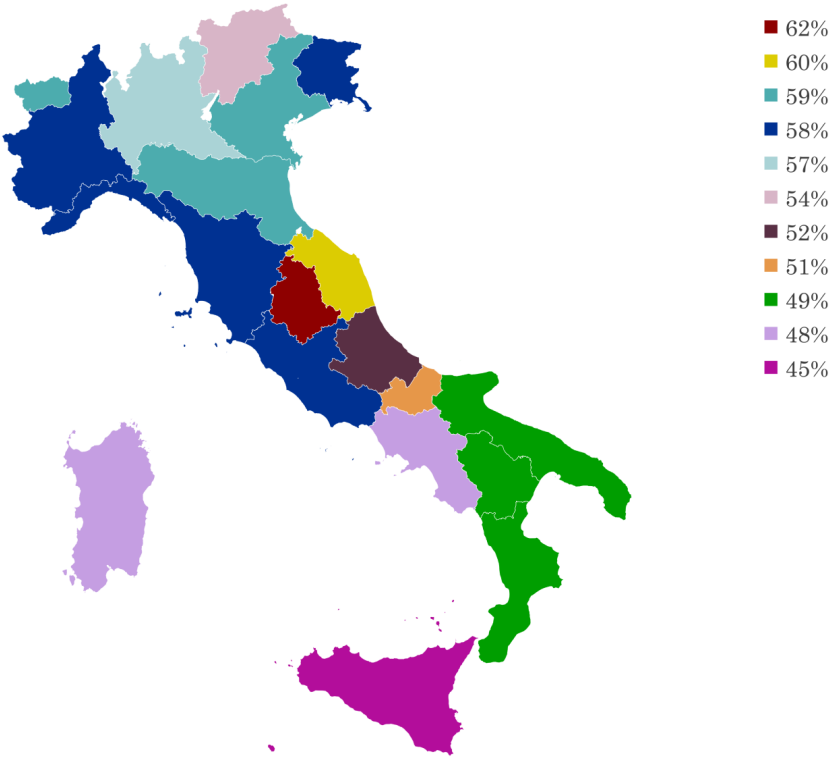
\includegraphics[width=.62\textwidth]{images/grafico_consumatori_regioni.png}
\end{center}
\noindent Dall'analisi del grafico sottostante emerge chiaramente un notevole aumento del consumo di vino da parte dei giovani. Questa tendenza rappresenta un'opportunità significativa per il settore vinicolo, in quanto indica un cambiamento nelle preferenze e nei comportamenti dei consumatori più giovani.\meskip
L'aumento del consumo di vino tra i giovani suggerisce un crescente interesse per la cultura enologica, la scoperta di nuovi sapori e l'esperienza di bevande di alta qualità. Tale tendenza potrebbe essere attribuita a una maggiore consapevolezza dei giovani sui benefici del vino, come le proprietà antiossidanti e la sua associazione con uno stile di vita sofisticato.\meskip
È quindi essenziale adattarsi a questa tendenza, offrendo una selezione di vini adatta ai gusti e alle preferenze dei giovani, utilizzando strategie di marketing mirate e coinvolgenti per catturare l'attenzione di questo segmento di mercato in crescita.\smallskip
\begin{center}
    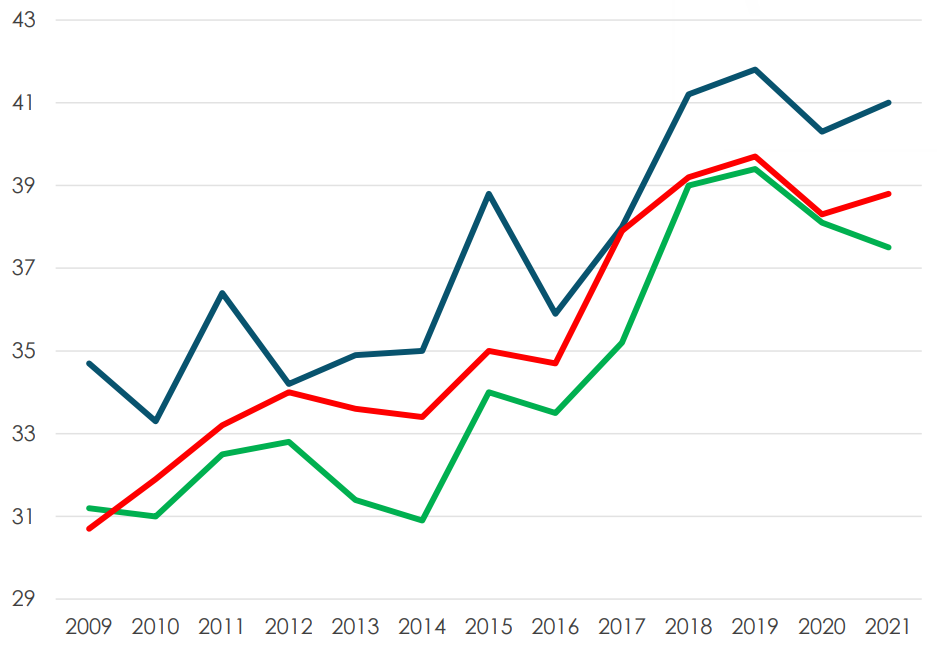
\includegraphics[width=.85\textwidth]{images/consumo_vino_eta.png}
\end{center}
La fascia di consumatori compresa tra i 30 e i 45 anni manifesta un forte interesse per tutti gli aspetti della sostenibilità, inclusi quelli ambientali, economici e sociali. Questi consumatori attribuiscono grande importanza alla provenienza etica dei vini, alle pratiche agricole sostenibili e alla responsabilità sociale delle aziende vinicole. La sostenibilità diventa quindi un fattore decisivo nella scelta dei vini per questa fascia di età.\meskip
D'altra parte, i giovani compresi tra i 18 e i 25 anni mostrano una particolare attrazione verso i vini di prestigio e riconosciuti a livello di brand. Tuttavia, sono anche alla ricerca di nuove esperienze e sono fortemente influenzati dagli eventi e dalle fiere del settore. Questa fascia di consumatori è attiva sui social media, dove seguono influencer del settore vinicolo e cercano informazioni su nuovi vini. È interessante notare che i giovani consumatori, se colpiti positivamente da un vino, tendono a voler approfondire l'esperienza, visitando direttamente le cantine.\meskip
Le donne, in particolare nella fascia di età compresa tra i 30 e i 45 anni, rappresentano oltre il 40\% degli iscritti a degustazioni e corsi di assaggio, ma sono anche la fascia di età che maggiormente apprezza e partecipa a visite aziendali e si avvale dei servizi legati all'Enoturismo.\meskip
Le donne hanno dimostrato una partecipazione attiva nel mondo del vino, sia in termini di formazione sia in termini di esperienze pratiche. Sono sempre più coinvolte in degustazioni guidate, corsi di assaggio e percorsi formativi per approfondire le loro conoscenze sul vino.

\subsection{Analisi PEST}

\subsubsection*{Fattori politici}
Vinovo opera in un'area geografica limitata all'Italia, il che presenta un vantaggio in quanto deve rispettare solo la legislazione nazionale.
La vendita di prodotti online non è soggetta a restrizioni significative, il che semplifica l'ingresso nel mercato, ma allo stesso tempo genera preoccupazione per la facilità con cui nuovi concorrenti potrebbero guadagnare quote di mercato.\\
In Italia, i siti web specializzati nella vendita online devono seguire una specifica normativa fiscale:
\begin{itemize}[itemsep=-5pt, topsep=0pt]
    \item aprire una partita IVA registrandosi presso la Camera di Commercio
    \item le informazioni dell'azienda devono essere chiaramente visibili sul portale online, consentendo agli utenti di trovare facilmente dati come il numero di partita IVA, l'indirizzo della sede legale e il codice di registrazione al Registro delle Imprese.
    \item si deve utilizzare il sistema di fatturazione elettronica, che prevede l'archiviazione digitale delle fatture per un periodo di 10 anni.
\end{itemize}

\subsubsection*{Fattori economici}
È importante tenere in considerazione il cambiamento climatico il quali potrebbe portare a difficoltà e quindi una riduzione significativa della produzione di uva in Italia.\\
Questa riduzione della quantità di uva disponibile potrebbe portare a un aumento dei costi di produzione per le aziende vinicole, in quanto l'offerta di uva è diminuita.\\
Se allo stesso tempo, supponiamo ci sia una crescente domanda di vini italiani all'estero, questo potrebbe portare a un aumento dei prezzi dei vini italiani sul mercato internazionale.
Di conseguenza, le aziende vinicole italiane potrebbero trovarsi ad affrontare costi di produzione più elevati a causa della riduzione dell'offerta di uva e potrebbero anche decidere di aumentare i prezzi dei loro vini per sfruttare la domanda crescente sui mercati internazionali.
Dunque è fondamentale instaurare forti collaborazioni con le aziende vinicole e soprattutto piccoli fornitori.

\subsubsection*{Fattori sociali}
Le preferenze dei consumatori italiani per il vino possono variare in base alle tradizioni regionali, alle abitudini alimentari e alle tendenze di consumo. Vinovo deve adattarsi alle preferenze dei clienti italiani e offrire una gamma di vini che risponda alle diverse esigenze e agli stili di vita dei consumatori locali.\\
Inoltre l'Italia è nota per la sua cultura enogastronomica, e Vinovo può sfruttare l'interesse dei consumatori per i vini italiani di qualità, promuovendo la provenienza, la tradizione e la varietà dei vini offerti.

\subsubsection*{Fattori tecnologici}
In Italia, l'innovazione tecnologica nel settore dell'e-commerce, come miglioramenti nella sicurezza dei pagamenti online, nell'esperienza di acquisto e nella logistica di consegna, influiscono sulla facilità con cui i consumatori possono acquistare vino online.
L'adozione di strumenti digitali e soluzioni tecnologiche nel settore vinicolo può influenzare la competitività della nostra proposta. Ad esempio, l'utilizzo di strumenti di analisi dei dati per comprendere meglio i comportamenti dei clienti e offrire raccomandazioni personalizzate può contribuire al successo di Vinovo.\bigskip
\begin{center}
    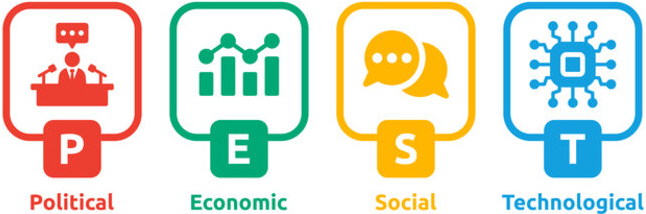
\includegraphics[width=.6\textwidth]{images/pest-analisys.png}
\end{center}

\subsection{Analisi dell'offerta}
In Italia, il mercato del vino è caratterizzato da numerosi produttori privati e piccole enoteche che tradizionalmente vendono i loro prodotti esclusivamente attraverso negozi fisici. Tuttavia, per queste realtà, avviare un proprio e-commerce rappresenta una sfida economica non sostenibile. Di conseguenza, spesso si affidano a piattaforme online già esistenti per raggiungere una clientela più ampia e sfruttare le opportunità offerte dal commercio digitale.

\subsubsection{Analisi dei concorrenti}
Per determinare la quota di mercato che possiamo ottenere, è fondamentale tenere presente che questo segmento di mercato è dominato da aziende consolidate, che vantano un notevole potere di contrattazione sia nei confronti dei clienti che dei fornitori. Nonostante queste sfide, siamo pronti ad affrontare la competizione con innovazione e determinazione. Siamo pronti a sfidare i giganti e a conquistare il nostro spazio nel mercato.\meskip
Sono stati individuati cinque principali concorrenti: Callmewine, Vine.com, Tannico, Xtrawine e Bernabei. Successivamente verranno fornite brevi descrizioni e confronti tra di loro, nonché anche con la nostra startup.\meskip
L'obiettivo è quello di sviluppare una strategia che soddisfi le esigenze dei clienti e offra servizi unici non ancora forniti dai nostri principali concorrenti. Inoltre, l'analisi della concorrenza sarà un processo continuo per rimanere sempre aggiornati e in grado di adattarci al mercato in evoluzione.\meskip
La tabella qui di seguito riassume i principali elementi che distinguono Vinovo dai concorrenti sopra citati:\meskip
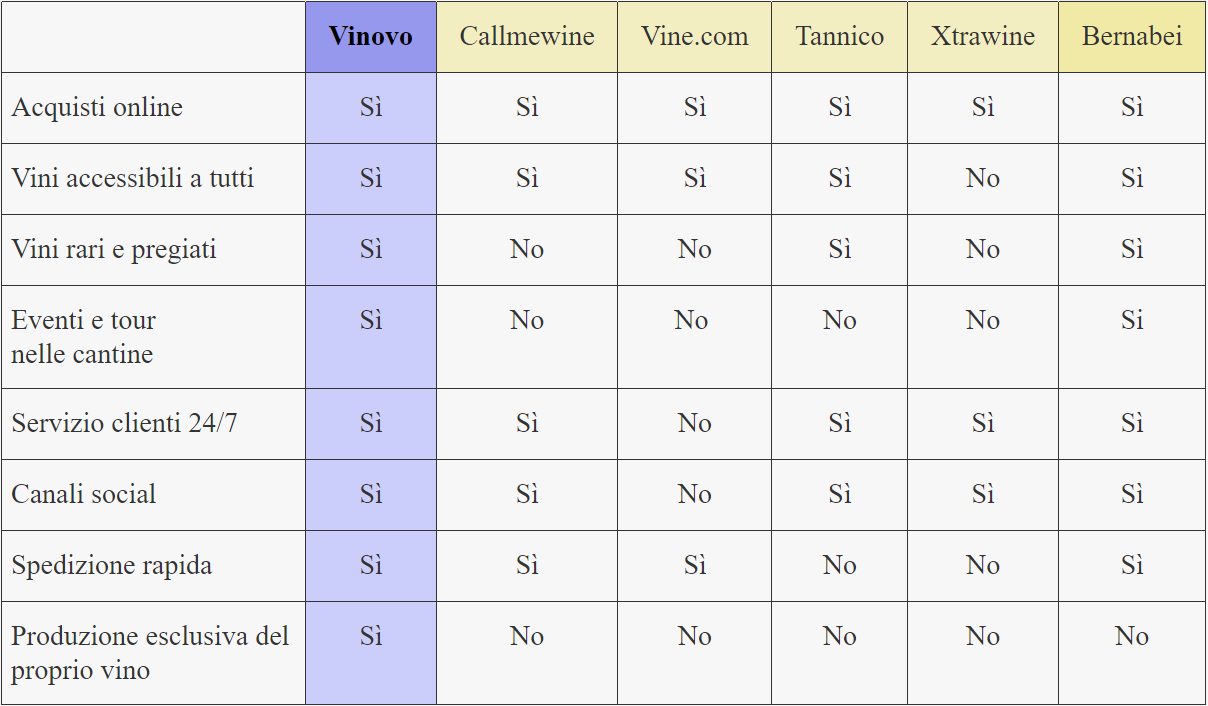
\includegraphics[width=\textwidth]{images/tabella_competitors.png}

\begin{itemize}
    \item \textbf{Callmewine}, è una piattaforma di e-commerce specializzata nella vendita di vini che si colloca tra i leader di mercato in Italia. Possiede un ampio catalogo con circa 11.000 etichette disponibili, che spaziano dai grandi nomi del panorama enologico mondiale ai piccoli produttori, dai distillati di brand più noti a quelli più di nicchia. Possiede quindi una selezione vasta ed eterogenea riuscendo però a guidare l'utente in una scelta consapevole senza disorientarlo, proprio come un vero "sommelier personale".
    \item \textbf{Vino.com} ha lanciato una piattaforma proprietaria multi-brand e multi-channel che ha modernizzato i processi di distribuzione di vino. Oggi \textit{Vino.com} presenta un catalogo di oltre 1.000 cantine e più di 6.000 etichette nazionali e internazionali e il suo fatturato 2020 ha raggiunto i 30 milioni di euro.
    \item \textbf{Tannico} è una delle più ampie enoteche online per offerta di vini italiani nel mondo, con più di 15.000 etichette. Le bottiglie, conservate nel magazzino di Milano, vengono spedite fino a 20 paesi in Europa, e non solo, e provengono da 2.500 cantine attentamente selezionate. Tecnologia, coraggio, innovazione, passione e visione, questi sono i valori con cui l'azienda descrive se stessa e su cui basa il proprio business, con la mission di "raccontare il vino con un linguaggio nuovo".
    \item \textbf{Xtrawine} è un'azienda nata dalla collaborazione di un gruppo di amici sommelier e informatici. Ormai consolidata sul mercato, lo testimoniano le oltre 10.000 referenze e una sede a Hong-kong che proietta le cantine sul mercato cinese; il tutto direttamente dalla piccola città di Forlì.
    \item \textbf{Bernabei} è un enoteca fisica e digitale; conta 5 enoteche fisiche, 5 wine corner e un ottimo e-commerce dove poter comprare oltre al vino, birre, spirits e bibite. Merita particolare attenzione la sezione Caveau con vini rari al suo interno e anche la parte di esperienze: una sezione che ti permette, acquistando il vino di determinate cantine, di poter andare a fare la visita con degustazione gratuitamente in loco.
\end{itemize}
Per concludere l'analisi, è essenziale sottolineare l'importanza dell'attività di differenziazione per mantenere una posizione competitiva nel mercato. Innanzitutto, offrire una spedizione rapida risulta fondamentale non solo per attrarre i clienti più esigenti, ma anche per garantire affidabilità ai ristoranti e locali che collaborano con noi.\meskip
Inoltre, uno dei nostri principali punti di forza è l'esclusività dei nostri vini. Essi vengono prodotti con cura e attenzione dopo un'accurata selezione della materia prima, oltre all'utilizzo di strumentazione all'avanguardia. Questo ci consente di offrire prodotti unici sul mercato, che soddisfano le aspettative dei nostri clienti più esigenti.\meskip
Infine, guardando al futuro, abbiamo l'obiettivo di diversificare le aree geografiche in cui produciamo i nostri vini, al fine di ridurre l'impatto ambientale dei trasporti. Questa strategia ci permetterà di sfruttare le risorse locali e di creare una catena di approvvigionamento più sostenibile, riducendo le distanze di trasporto e promuovendo un'impronta ecologica più ridotta.\bskip
In sintesi, attraverso l'offerta di spedizioni rapide, l'esclusività dei nostri vini e l'attenzione all'impatto ambientale, miriamo a distinguerci nel mercato e a garantire il successo a lungo termine della nostra attività.

\section{Business Model}
In questo capitolo viene presentato il Modello di Business di Vinovo, illustrando la logica fondamentale che ha portato alla creazione del progetto imprenditoriale e la strategia da implementare attraverso strutture organizzative, processi e sistemi, al fine di ottenere un vantaggio competitivo che consenta all'azienda di generare, distribuire e valorizzare i propri prodotti o servizi.

\subsection{Business Model Canvas}
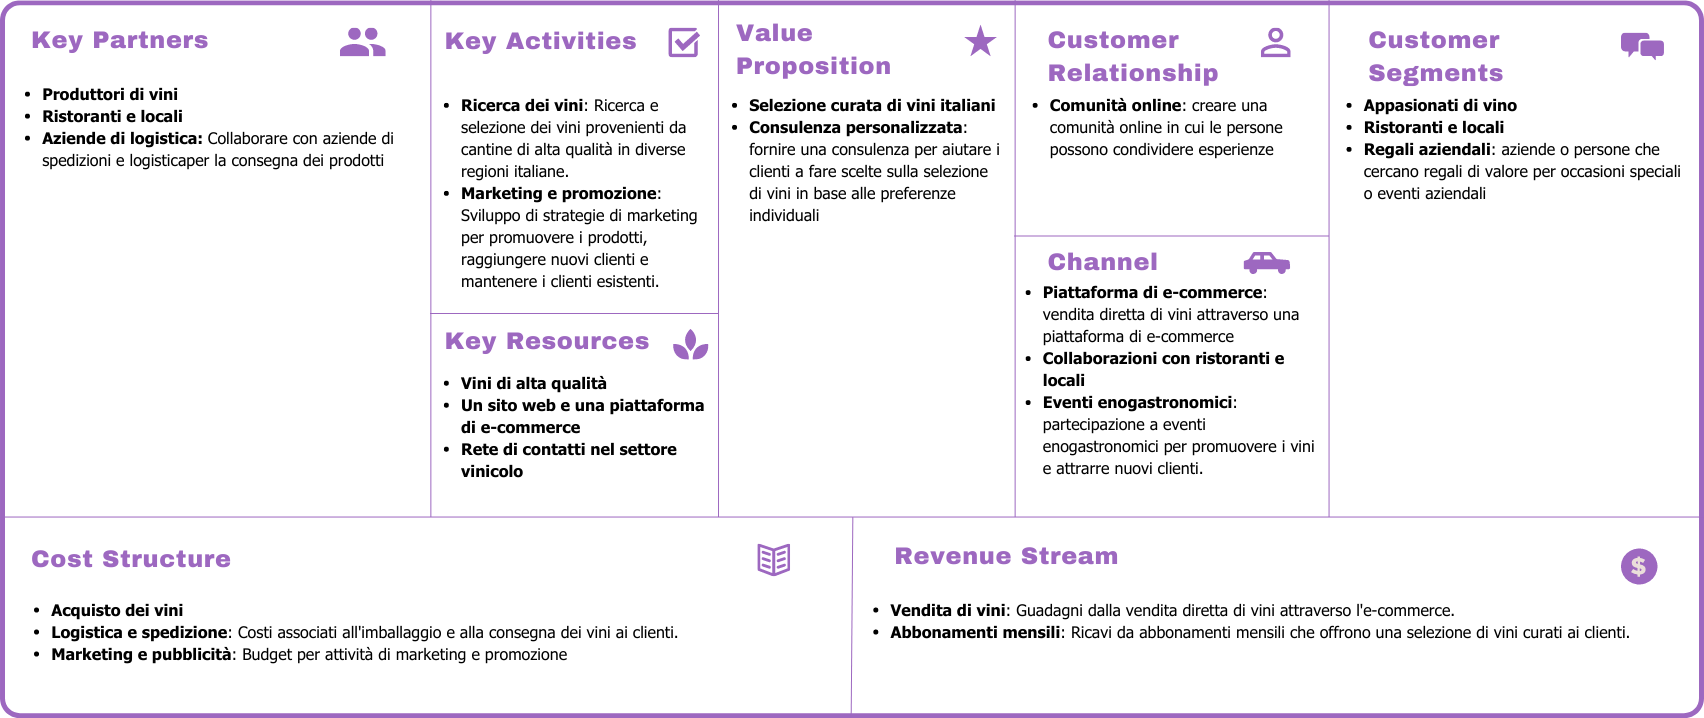
\includegraphics[width=\textwidth]{images/business_model_canvas.png}

\subsubsection{Key Partners}
La rete di collaborazioni di Vinovo rappresenta una componente fondamentale del suo modello di business, consentendo a Vinovo di fornire un servizio completo e soddisfacente ai clienti.
\begin{itemize}
    \item \textbf{Produttori e distributori di vino}: stabilire relazioni solide con produttori e distributori di vino è fondamentale per ottenere una vasta selezione di vini di qualità da offrire ai clienti. Collaborare con fornitori affidabili e di buona reputazione aiuterà a garantire un assortimento vario e interessante.
    \item \textbf{Corrieri}: lavorare con corrieri specializzati nel trasporto di bevande alcoliche consentirà di garantire la consegna sicura e puntuale dei prodotti ai clienti. Assicurati di trovare partner logistici che comprendano le esigenze specifiche delle bevande alcoliche e siano in grado di gestire l'invio di bottiglie di vino in modo adeguato.
    \item \textbf{Fornitori di imballaggi}: trovare fornitori di imballaggi adeguati e sicuri per le bottiglie di vino è importante per proteggere i prodotti durante il trasporto.
    \item \textbf{Piattaforme di pagamento}: integrare un sistema di pagamento sicuro e affidabile è essenziale per consentire ai clienti di effettuare transazioni online in sicurezza. Collaboriamo con provider di servizi di pagamento rinomati per offrire opzioni di pagamento convenienti e protette.
          % \item \textbf{Esperti di vino e sommelier}: collaborare con esperti di vino, sommelier o enologi può apportare un grande valore, possono fornire consulenze sulla selezione dei vini, descrizioni dettagliate dei prodotti e offrire consigli personalizzati ai clienti.
          % \item \textbf{Specialisti di marketing e pubblicità}: lavorare con professionisti del settore del marketing digitale e della pubblicità; collaborare con agenzie di marketing per creare strategie pubblicitarie, gestire campagne di social media e aumentare la visibilità.
          % \item \textbf{Partner di e-commerce}: la possibilità di collaborare con piattaforme di e-commerce esistenti, come siti web specializzati nella vendita di vini o marketplace di prodotti alimentari e bevande. Questa partnership permette di aumentare la visibilità online.
\end{itemize}

\subsubsection{Key Activities}
Di seguito sono riportate non solo le principali attività proposte nel Busness Model Canvas, ma anche attività di secondaria importanza:
\begin{itemize}
    \item \textbf{Ricerca dei vini}: Identificare, selezionare e acquisire una varietà di vini provenienti da diverse regioni e produttori. Stabilire partnership con fornitori affidabili per garantire una selezione di vini di alta qualità.
    \item \textbf{Creazione di una piattaforma di e-commerce}: Sviluppo e gestione un sito web per consentire agli utenti di esplorare il catalogo di vini, effettuare ordini e pagamenti online in modo sicuro.
    \item \textbf{Gestione dell'inventario}: Mantenere un inventario accurato dei vini disponibili, gestire la logistica e il magazzino per garantire la pronta consegna degli ordini.
    \item \textbf{Marketing e promozione}: Creare strategie di marketing online per promuovere il marchio Vinovo e attirare potenziali clienti. Utilizzare canali di comunicazione come i social media e la pubblicità online per aumentare la visibilità dell'azienda.
    \item \textbf{Servizio clienti}: Offrire un servizio clienti di alta qualità per rispondere alle domande degli utenti, fornire assistenza nella scelta dei vini e gestire eventuali problemi o reclami. Mantenere una comunicazione tempestiva ed efficace tramite chat online o e-mail.
          % \item \textbf{Logistica e spedizioni}: Organizzare la logistica e la spedizione dei prodotti in modo efficiente, in collaborazione con corrieri o società di consegna, per garantire consegne tempestive e affidabili ai clienti.
          % \item \textbf{Gestione delle partnership}: Stabilire e gestire relazioni con i produttori di vino e altri partner nel settore per garantire l'approvvigionamento regolare dei vini e sviluppare collaborazioni strategiche per ampliare la gamma di prodotti offerti.
    \item \textbf{Monitoraggio e analisi dei dati}: Raccogliere e analizzare dati relativi alle vendite, al comportamento dei clienti e alle preferenze di consumo per identificare tendenze di mercato, migliorare l'offerta di prodotti e ottimizzare le strategie di marketing.
    \item \textbf{Ricerca e sviluppo}: Restare aggiornati sulle nuove tendenze e innovazioni nel settore vinicolo, esplorare nuove opportunità di prodotto e migliorare costantemente l'offerta di Vinovo per rimanere competitivi sul mercato.
          % \item \textbf{Gestione finanziaria}: Monitorare le finanze dell'azienda, compresa la gestione del flusso di cassa, l'elaborazione dei pagamenti dei clienti e la gestione delle spese operative.
\end{itemize}



\subsubsection{Key Resources}
Vinovo basa la propria forza su tre risorse fondamentali:
\begin{itemize}
    \item \textbf{Qualità dei prodotti}:\\
          La prima risorsa è la qualità dei prodotti. Vinovo si distingue per la produzione di vini di alta qualità. Grazie alla conoscenza e all'esperienza nella vinificazione, l'azienda crea prodotti che soddisfano i palati più raffinati, con caratteristiche uniche di sapore, aroma e complessità. Dalla selezione delle uve alla fase di fermentazione e all'invecchiamento, ogni dettaglio è curato con attenzione per ottenere vini di eccellenza.
    \item \textbf{Comunicazione e presenza online}:\\
          La comunicazione con i clienti e la presenza online costituiscono un'altra risorsa cruciale per Vinovo. Consapevole del crescente ruolo di internet nelle decisioni di acquisto, l'azienda ha sviluppato un sito web e una piattaforma e-commerce all'avanguardia. Il sito web offre informazioni dettagliate sulle varietà di vino offerte, la storia dell'azienda e le recensioni dei clienti, costruendo fiducia e rafforzando l'immagine di un marchio affidabile. Inoltre, la piattaforma e-commerce consente ai clienti di effettuare ordini comodamente da casa, espandendo il mercato potenziale e semplificando la distribuzione dei prodotti.
    \item \textbf{Partner unici e rete di contatti}:\\
          Infine, Vinovo beneficia di una rete di contatti nel settore vinicolo che rappresenta una risorsa di grande valore. Queste partnership offrono opportunità di collaborazione, scambio di conoscenze e nuovi canali di vendita. Partecipare a eventi di settore, fiere del vino e degustazioni consente a Vinovo di creare nuovi contatti e di interagire con professionisti che contribuiscono alla crescita e al successo dell'azienda.
\end{itemize}
In conclusione, la qualità dei prodotti, la presenza online ben curata e la rete di contatti nel settore vinicolo rappresentano risorse essenziali. Sfruttando al meglio queste risorse, l'azienda ottiene visibilità, espande il proprio mercato e costruisce una reputazione solida, permettendo di prosperare in un settore altamente competitivo.

\subsubsection{Value Proposition}
Vinovo si distingue per la \textbf{produzione interna ed esclusiva} dei suoi vini, che rappresentano il suo punto di forza. La passione e l'esperienza del team enologico si riflettono in ogni bottiglia, garantendo un gusto unico. Ogni fase del processo di produzione, dalla coltivazione delle viti all'imbottigliamento, avviene direttamente presso le tenute di Vinovo, consentendo un controllo rigoroso su ogni dettaglio e mantenendo intatta l'autenticità dei prodotti. Grazie a questa filosofia vinicola intraprendente, Vinovo si posiziona come un punto di riferimento per gli appassionati del buon vino, offrendo una gamma esclusiva di etichette.\meskip
Inoltre, di seguito sono elencate ulteriori proposte di valore che completano l'esperienza dei suoi vini:
\begin{itemize}
    \item \textbf{Vasta selezione di vini:} La start-up si distingue per la varietà e l'originalità della selezione, consentendo ai clienti di scoprire e acquistare vini unici e di alta qualità.
    \item \textbf{Qualità e autenticità:} Garantire che tutti i vini offerti siano autentici e di elevata qualità, fornendo informazioni riguardanti la provenienza, la produzione e la selezione dei vini per garantire ai clienti un'esperienza degustativa superiore.
    \item \textbf{Esperienza di acquisto online conveniente:} Offrire ai clienti un'esperienza di acquisto online facile e conveniente, consentendo loro di sfogliare l'assortimento di vini, leggere descrizioni dettagliate, confrontare prezzi e fare acquisti in modo semplice e sicuro dal comfort di casa loro.
          % \item \textbf{Consegna affidabile}: Garantire una consegna sicura e puntuale dei vini ai clienti. Ciò include un imballaggio adeguato per proteggere le bottiglie durante il trasporto e la collaborazione con corrieri specializzati nel settore delle bevande alcoliche per garantire una gestione adeguata delle spedizioni.
    \item \textbf{Esperienza enogastronomica:} Offrire non solo la vendita di vini, ma anche la promozione dell'esperienza enogastronomica. Fornire informazioni sulle regioni vinicole, le uve utilizzate nella produzione dei vini e suggerimenti di abbinamento con cibi specifici per arricchire l'esperienza dei clienti.
    \item \textbf{Offerte esclusive e accesso privilegiato:} Offrire ai clienti accesso a offerte esclusive, come vini rari o limitati, ed eventi speciali come degustazioni o visite a cantine. Questo creerà un senso di privilegio e appartenenza per i clienti, incentivando la fedeltà e la partecipazione alla comunità di Vinovo.
    \item \textbf{Servizio clienti di qualità:} Fornire un'eccellente assistenza clienti, rispondendo prontamente alle domande e alle richieste dei clienti, offrendo supporto post-vendita e risolvendo eventuali problemi in modo tempestivo ed efficace.
\end{itemize}

\subsubsection{Customer Relationship}
Per Vinovo, la creazione e il mantenimento di una relazione solida con i nostri clienti è di fondamentale importanza per il nostro successo. Vogliamo dimostrare loro autenticità, trasparenza e affidabilità, offrendo un servizio eccellente in ogni momento.
Crediamo fermamente nell'importanza di stabilire un legame autentico con i nostri clienti. Per fare ciò, raccogliamo informazioni sui loro gusti e preferenze, in modo da offrire consigli e suggerimenti personalizzati. Ci sforziamo di creare un'esperienza di acquisto personalizzata che rispecchi i loro desideri.\\
La trasparenza è un valore fondamentale per noi. Comunichiamo apertamente con i nostri clienti riguardo ai nostri prodotti, alla loro provenienza e alle pratiche di produzione. Desideriamo che i nostri clienti siano pienamente informati sulle caratteristiche dei vini che offriamo, in modo che possano prendere decisioni consapevoli e fidarsi della nostra azienda.\\
L'affidabilità è alla base del nostro impegno per fornire un servizio di qualità. Siamo pronti a rispondere prontamente alle domande e alle preoccupazioni dei nostri clienti. Mettiamo a disposizione diverse modalità di assistenza, come chat ed e-mail, per assicurare che le esigenze dei nostri clienti vengano soddisfatte in modo efficiente. Vogliamo superare le loro aspettative e risolvere i loro problemi nel miglior modo possibile. \qquad
Inviamo regolarmente aggiornamenti e newsletter per tenerli informati sulle nostre offerte speciali, nuovi arrivi e eventi, offrendo contenuti interessanti e utili che vanno oltre la semplice vendita.


\subsubsection{Channel}
Al fine di interagire coi clienti, Vinovo possiede una piattaforma online che, una volta effettuata la registrazione, permette ai clienti di acquistare i prodotti desiderati direttamente dalla piattaforma, aggiungendoli al carrello nella quantità desiderata.\\
Inoltre, la start-up fornisce ai clienti informazioni immediate sulla data di consegna prevista e offre il servizio di tracciamento della spedizione, permettendo loro di monitorare il percorso del pacco.\\
Per quanto riguarda le modalità di pagamento, Vinovo offre diverse opzioni. Queste includono il pagamento con carta di credito e l'utilizzo del servizio di pagamento online Paypal, che garantisce un'ulteriore sicurezza nelle transazioni.\\
Al fine di raggiungere una vasta gamma di clienti e promuovere il proprio marchio, Vinovo ha integrato i social media nella sua strategia comunicativa. Questi canali aggiuntivi permettono all'azienda di raggiungere un ampio bacino di utenti, offrendo contenuti interessanti, promozioni e coinvolgendo attivamente la comunità degli appassionati di vino. L'utilizzo dei social media contribuisce ad aumentare la visibilità e favorire l'interazione con i clienti.\meskip
La start-up partecipa attivamente a eventi enogastronomici come fiere, degustazioni, festival o eventi dedicati al vino. Questi eventi forniscono un'opportunità per promuovere i vini della start-up, mettere in mostra la qualità dei propri prodotti e creare connessioni dirette con i potenziali clienti. Partecipando a eventi enogastronomici, l'azienda può attrarre nuovi clienti interessati al mondo del vino.

\subsubsection{Customer Segments}
\begin{itemize}
    \item \textbf{Appassionati di vino}: Questo segmento comprende gli amanti del vino che apprezzano la qualità, la varietà e l'esperienza di scoprire nuovi vini. Sono interessati a prodotti unici, selezionati con cura e potrebbero essere disposti a spendere di più per ottenere vini di alta qualità.
    \item \textbf{Ristoranti e locali}: I ristoranti, le enoteche e gli altri locali che offrono una selezione di vini possono essere un segmento di clientela interessante per Vinovo. Offrire loro un'ampia scelta di vini e la comodità di ordinare online potrebbe semplificare la gestione del loro inventario e soddisfare i loro clienti.
    \item \textbf{Regali aziendali}: Le aziende spesso cercano regali speciali per i propri clienti, partner commerciali o dipendenti. Vinovo potrebbe creare offerte personalizzate per regali aziendali, sarà possibile scegliere sul sito se spedire il prodtto già impacchettato come regalo.
    \item \textbf{Regali personali}: Non solo aziende, ma anche semplicemente un regalo per occasioni speciali come compleanni e matrimoni.
          % \item \textbf{Clienti internazionali}: Grazie alla natura dell'e-commerce, Vinovo può espandersi e raggiungere clienti internazionali che sono interessati a scoprire e acquistare vini provenienti da diverse regioni del mondo. Adattare la piattaforma per supportare spedizioni internazionali e offrire informazioni dettagliate sulle etichette e le regioni vinicole può attirare questa clientela.
    \item \textbf{Clienti in cerca di convenienza}: Vinovo può rivolgersi a clienti che apprezzano la comodità dell'acquisto online e della consegna a domicilio. Questo segmento di clientela cerca un'esperienza di acquisto facile e senza problemi.
\end{itemize}

\subsubsection{Cost Structure}
\begin{itemize}
    \item \textbf{Acquisto di vini}: Questo è il costo principale per la start-up. Bisogna acquistare una varietà di vini dai produttori per costruire l'inventario. Costo dipenderà dalla qualità e dalla quantità dei vini che si decide di acquistare.
    \item \textbf{Logistica e spedizioni}: La gestione delle spedizioni dei vini richiede attenzione particolare, poiché è necessario garantire che le bottiglie siano ben imballate e consegnate in modo sicuro. Ci saranno costi associati all'imballaggio, alle etichette di spedizione, ai servizi di corriere e alle tariffe di spedizione nazionali.
    \item \textbf{Marketing e pubblicità}: Per promuovere l' attività e attirare clienti, si dovrà investire in attività di marketing e pubblicità. Ciò può includere la creazione di contenuti promozionali, la gestione di campagne pubblicitarie online, la partecipazione a eventi di settore o magari la collaborazione con influencer del settore.
    \item \textbf{Gestione del sito web e sviluppo}: Bisogna considerare i costi di sviluppo, progettazione e manutenzione del sito. Ci possono essere costi associati all'acquisto di un dominio, all'hosting del sito, alle tariffe del sistemi di pagamento.
    \item \textbf{Servizio clienti}: Investire nella gestione del servizio clienti è importante per garantire un'esperienza di acquisto positiva. Ciò può includere la formazione del personale, l'utilizzo di strumenti di supporto clienti, l'implementazione di sistemi di chat online e l'assegnazione di risorse per gestire le domande e le richieste dei clienti.
\end{itemize}

\subsubsection{Revenue Streams}
\begin{itemize}
    \item La \textbf{Vendita diretta di vini} attraverso la piattaforma di e-commerce sarà il principale flusso di ricavi per Vinovo.
    \item \textbf{Abbonamenti}: Un'opzione per Vinovo potrebbe essere creare un servizio di abbonamento che offre ai clienti una selezione periodica di vini, offerte esclusive e l'opportunità di scoprire nuove etichette. Questo può attirare clienti che desiderano esplorare e ricevere una selezione regolare di vini.
    \item \textbf{Vendita di accessori e prodotti correlati}: Oltre alla vendita di vini, si intende aggiungere anche altri accessori per il vino, come bicchieri, caraffe, cavatappi e altre attrezzature collegate al mondo del vino. Questa espansione della nostra proposta commerciale non solo completerà l'esperienza dei nostri clienti, ma ci offrirà anche un flusso di ricavi supplementare. Con l'aggiunta di questi prodotti correlati, vogliamo offrire un'esperienza ancora più completa, in cui i nostri clienti potranno trovare tutto ciò di cui hanno bisogno direttamente con Vinovo.
    \item \textbf{Collaborazioni e partnership}: Abbiamo l'intenzione di stabilire collaborazioni strategiche con ristoranti e locali al fine di creare offerte o pacchetti speciali. Attraverso queste partnership, miriamo a condividere i ricavi derivanti dalle vendite.
    \item \textbf{Eventi e degustazioni}: Organizzare eventi di degustazione di vini e generare ricavi attraverso la vendita di biglietti. Questi eventi possono aiutare a promuovere il tuo marchio e fornire un'esperienza coinvolgente ai clienti.\\ Inizialmente, abbiamo deciso di offrire l'accesso gratuito ai nostri eventi. Tuttavia, una volta che l'azienda avrà consolidato il suo valore e sviluppato ulteriormente le sue offerte, prevediamo di introdurre una tariffa. Questo passaggio a un modello a pagamento ci permetterà di alzare gli standard e offrire servizi e contenuti ancora più esclusivi e curati. Ciò ci consentirà di investire ulteriormente nell'organizzazione degli eventi, garantendo una miglior esperienza.

\end{itemize}

\section{Marketing}
La funzione Marketing della nostra start-up Vinovo gioca un ruolo fondamentale nel posizionamento del nostro marchio sul mercato e nella creazione di una base solida di clienti. Il nostro obiettivo è promuovere i nostri prodotti enogastronomici in modo da attirare l'attenzione del pubblico di riferimento e aumentare la consapevolezza del marchio.\\
Di seguito sono descritte le principali attività e strategie che implementeremo per raggiungere questi obiettivi.
\begin{itemize}
    \item \textbf{Ricerca di mercato}: Prima di lanciare il nostro servizio di vendita online, condurremo una ricerca di mercato approfondita per comprendere meglio i desideri, le preferenze e le abitudini di consumo del nostro target di clientela. Analizzeremo anche la concorrenza per identificare opportunità uniche di posizionamento e differenziazione.\\ Vedi capitolo 2.
    \item \textbf{Segmentazione di mercato}: Utilizzeremo i risultati della ricerca di mercato per suddividere il nostro pubblico di riferimento in diversi segmenti; questo ci permetterà di personalizzare le nostre strategie di marketing e comunicazione per raggiungere gruppi specifici di clienti con pubblicità mirata.
          % \item Posizionamento del marchio: Definiremo una chiara proposta di valore per il nostro marchio Vinovo, identificando i suoi punti di forza distintivi e unici. Comunicheremo in modo efficace tali caratteristiche distintive ai nostri potenziali clienti per creare un'immagine di marca positiva e differenziata.
    \item \textbf{Strategie di promozione}: Utilizzeremo un mix di strategie di promozione per aumentare la visibilità del marchio e attirare i clienti. Queste strategie includeranno la pubblicità online, le campagne sui social media e il coinvolgimento degli influencer del settore.
    \item \textbf{Sito web e presenza online}: Creeremo un sito web attraente e intuitivo che offra una piattaforma di vendita online user-friendly per i nostri clienti (Vedi capitolo 1). Ottimizzeremo il sito web per i motori di ricerca (SEO) in modo che sia facilmente trovabile dai potenziali clienti. Inoltre, gestiremo attivamente la nostra presenza sui social media per coinvolgere e interagire con i nostri follower.
    \item \textbf{Collaborazioni e partnership}: Cercheremo opportunità di collaborazione e partnership con influencer, blogger e altri attori rilevanti nel settore enogastronomico. Queste collaborazioni ci aiuteranno a espandere la nostra visibilità e ad ampliare il nostro pubblico di potenziali clienti.
          % \item Customer relationship management (CRM): Implementeremo un sistema CRM per gestire e tracciare le interazioni con i nostri clienti. Questo ci aiuterà a mantenere relazioni solide con i clienti esistenti e a fornire un servizio personalizzato basato sulle loro preferenze e necessità.
    \item \textbf{Monitoraggio e analisi delle performance}: Monitoreremo costantemente le performance delle nostre attività di marketing utilizzando metriche chiave come il tasso di conversione, il traffico sul sito web e l'engagement sui social media. Basandoci sui dati raccolti, apporteremo eventuali ottimizzazioni e miglioramenti alle nostre strategie di marketing per massimizzare i risultati.
          % \item La funzione Marketing sarà guidata da un team competente e appassionato che lavorerà in sinergia con gli altri reparti dell'azienda per garantire un'esperienza di marca coerente e di alta qualità. Siamo determinati a creare una presenza di marca forte e riconoscibile nel settore enogastronomico, posizionando Vinovo come una scelta preferita dai consumatori per i prodotti di qualità e l'eccellenza del servizio.
\end{itemize}\bigskip
Per valutare il grado di attrattività del settore in cui opera la nostra start-up Vinovo, è importante considerare diversi fattori che possono influenzare le prospettive di crescita, i margini di profitto e le opportunità di sviluppo nel settore enogastronomico.\\
Di seguito sono riportati alcuni aspetti chiave da prendere in considerazione:
\begin{itemize}
    \item \textbf{Dimensione e crescita del mercato}: Il settore enogastronomico è ampio e in continua crescita. La domanda di prodotti enogastronomici di alta qualità è in costante aumento. L'ampia base di clientela e la tendenza al consumo consapevole rappresentano un fattore positivo per il nostro business.
    \item \textbf{Competizione}: Il settore enogastronomico è altamente competitivo, con numerose aziende che offrono prodotti simili o complementari. La presenza di concorrenti consolidati può rappresentare una sfida, ma anche un'opportunità per differenziarsi e offrire un valore unico ai clienti.
    \item \textbf{Innovazione e tendenze di consumo}: L'innovazione è fondamentale nel settore enogastronomico, con continue evoluzioni nel campo delle tecniche di produzione e degli ingredienti. Seguire e anticipare le tendenze di consumo, come la preferenza per prodotti biologici e sostenibili, può favorire il successo del nostro business.
    \item \textbf{Regolamentazioni e normative}: Il settore enogastronomico è soggetto a diverse regolamentazioni e normative, ad esempio in materia di sicurezza alimentare, etichettatura e norme sanitarie. È importante garantire la conformità a tali requisiti per mantenere la fiducia dei clienti e operare in modo legale.
    \item \textbf{Fornitori}: La disponibilità di fornitori affidabili e di qualità è fondamentale per garantire l'approvvigionamento di prodotti freschi.
    \item \textbf{Evoluzione tecnologica}: Le nuove tecnologie stanno giocando un ruolo sempre più importante nel settore enogastronomico, ad esempio nell'e-commerce, nella gestione delle consegne e nelle esperienze digitali. Bisogna sfruttare queste opportunità al fine di raggiungere un pubblico più ampio.
    \item \textbf{Barriere all'ingresso}: Le barriere di ingresso nel settore enogastronomico online sono moderate. Al giorno d'oggi, lo sviluppo di un e-commerce ha costi molto accessibili. L'ostacolo più significativo sarà quello di creare una solida rete di produttori di alta qualità e ampliare i punti di stoccaggio per garantire una consegna rapida in tutta Italia in futuro.
\end{itemize}
Complessivamente, il settore enogastronomico offre ampie opportunità di crescita e successo per una start-up come Vinovo. Tuttavia, è fondamentale sviluppare una strategia di marketing ben strutturata, differenziarsi dalla concorrenza e mantenere un'attenzione costante alle esigenze dei clienti per sfruttare appieno il potenziale di attrattività del settore.

\subsection{Valutazione competitiva: le 5 forze di Porter}
Per valutare la propria posizione competitiva, si utilizza il modello delle 5 forze di Porter. Questo modello permette di individuare le forze che operano nell'ambiente economico, analizzandone l'intensità, l'importanza e il loro impatto sulla redditività a lungo termine delle aziende. Queste forze agiscono in modo continuo e, se non vengono adeguatamente monitorate, possono portare alla perdita di competitività. Pertanto, è fondamentale monitorarle attentamente e adottare le misure necessarie per contrastarle.
\begin{center}
    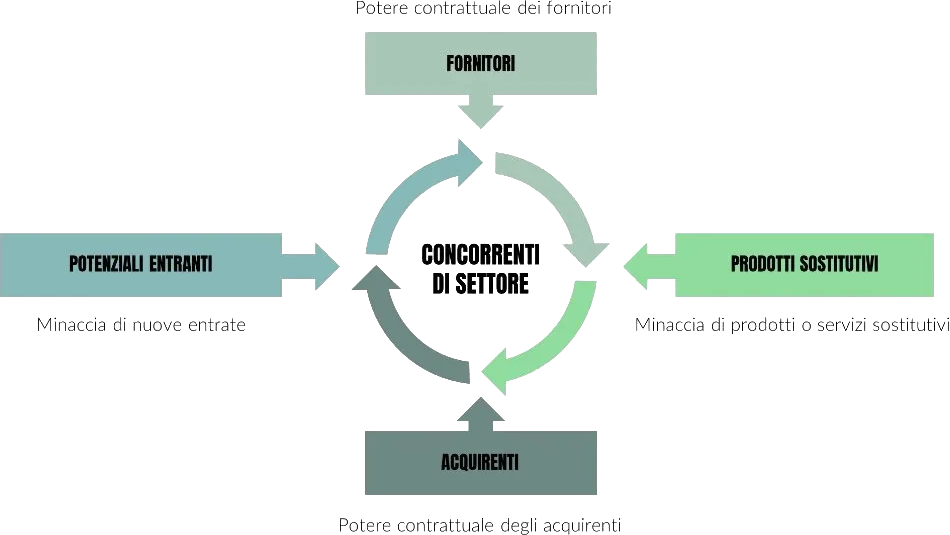
\includegraphics[width=\textwidth]{images/5-forze-di-porter.png}
\end{center}


\subsubsection{Minaccia di nuovi entranti}
La minaccia di nuovi entranti nell'industria dell'e-commerce del vino dipenderà da vari fattori. Ad esempio, se l'accesso ai canali di distribuzione e alle forniture di vino è relativamente facile, ci potrebbe essere una maggiore minaccia di nuove imprese che entrano nel mercato. Tuttavia, se riusciamo a chiudere accordi esclusivi con produttori di vino esterni e offrendo i nostri vini prodotti internamente, potremmo creare una barriera all'ingresso per i nuovi concorrenti.

\begin{itemize}
    \item \textbf{Accesso ai canali di distribuzione e alle forniture di vino}:
          Se l'accesso ai canali di distribuzione e alle forniture di vino è relativamente facile, ciò potrebbe abbassare le barriere all'ingresso per le nuove imprese. Tuttavia, se stabiliamo accordi esclusivi con produttori di vino o fornitori affidabili, potremmo ambire ad un vantaggio competitivo. Gli accordi esclusivi possono garantire l'accesso a vini unici, rari o di alta qualità, che potrebbero essere difficili da ottenere per i nuovi entranti. Ciò crea una barriera all'ingresso poiché i clienti potrebbero preferire Vinovo per la sua offerta unica.

    \item \textbf{Brand e reputazione}:
          La forza del marchio e la reputazione di Vinovo possono essere un fattore critico nella gestione della minaccia dei nuovi entranti. Puntiamo a stabilire una solida presenza online e una reputazione positiva nel settore, così da complicare l'ingresso ai concorrenti. La reputazione può essere costruita attraverso servizi clienti di alta qualità, recensioni positive, testimonianze e raccomandazioni da parte di esperti del settore. Un marchio ben consolidato può anche avere un vantaggio nell'acquisire nuovi clienti, poiché gli utenti potrebbero essere più inclini ad acquistare da un'azienda affermata e di fiducia.
\end{itemize}
In sintesi, l'ottenimento di accordi esclusivi con produttori di vino, sfruttando economie di scala nello stoccaggio e nella logistica, costruendo un marchio forte e una reputazione positiva nel settore. Questi fattori combinati mirano a complicare la barriera all'ingresso per i nuovi arrivati e consentono a Vinovo di mantenere una posizione competitiva nel mercato già esistente dell'e-commerce del vino.

\subsubsection{Minaccia di prodotti sostitutivi}
Diverse fonti potrebbero costituire una minaccia di prodotti sostitutivi per Vinovo:
\begin{itemize}
    \item \textbf{Prodotti alcolici alternativi}:\\
          La minaccia di prodotti sostitutivi per Vinovo deriva dalla disponibilità di alternative al vino, come birra, liquori o altre bevande alcoliche. I consumatori potrebbero preferire queste alternative a causa dei gusti personali, delle abitudini o dell'occasione sociale. Per affrontare questa minaccia, Vinovo potrebbe differenziare la sua offerta, concentrandosi su una vasta selezione di vini che offrano esperienze di degustazione e profili di gusto distinti.
    \item  \textbf{Esperienza di acquisto diretto}:\\
          Alcuni consumatori possono preferire l'acquisto di vino presso negozi fisici piuttosto che online, poiché desiderano toccare e vedere il prodotto prima dell'acquisto. È impossibile offrire lo stesso servizio online, ma possiamo minimizzare questo difetto andando ad includere informazioni dettagliate sui prodotti, comprese descrizioni del gusto, note di degustazione, informazioni sulla provenienza e suggerimenti di abbinamento cibo-vino. Inoltre, si potrebbe pensare alla vendita di campioni di prova, venduti in set di diverse tipologie di vino. Infine recensioni e testimonianze possono aiutare a costruire la fiducia dei consumatori.
\end{itemize}
Per affrontare la minaccia dei prodotti sostitutivi, Vinovo potrebbe anche concentrarsi sull'educazione dei consumatori e sul coinvolgimento nel mondo del vino. Questo può essere fatto attraverso blog, guide informative, video didattici o eventi che promuovono la conoscenza del vino, le varietà, i processi di produzione e gli abbinamenti. Inoltre, potremmo offrire consulenze personalizzate o programmi di abbonamento che consentono ai clienti di scoprire nuovi vini in base alle loro preferenze.

Attraverso collaborazioni e partnership, si potrebbe creare un valore aggiunto per i clienti e allo stesso tempo aumentare la visibilità di Vinovo. Ad esempio, Vinovo potrebbe offrire sconti esclusivi in alcuni ristoranti selezionati per i clienti che acquistano tramite la piattaforma Vinovo.\meskip
In sintesi, possiamo affrontare la minaccia dei prodotti sostitutivi attraverso la differenziazione dell'offerta di vini, l'offerta di un'esperienza di acquisto online informativa, l'educazione e il coinvolgimento dei consumatori.

\subsubsection{Potere contrattuale dei fornitori}
Il potere contrattuale dei fornitori dipende dalla nostra dipendenza nei confronti di determinati produttori di vino. Se ci basiamo su un numero limitato di fornitori o se i produttori di vino sono dominanti nel settore, potrebbero avere un maggiore potere contrattuale. In questo caso, i fornitori potrebbero imporre prezzi più alti o condizioni di fornitura meno favorevoli, poiché non abbiamo molte alternative.\meskip
È importante quindi adottare una strategia di diversificazione dei fornitori. Cercando di collaborare con un numero maggiore di produttori di vino e di ampliare la rete di approvvigionamento, ridurre quindi la dipendenza da singoli fornitori e avere maggiori opzioni di trattativa. In questo modo, se un fornitore diventa problematico o alza i prezzi in modo sproporzionato, abbiamo subito delle alternative pronte a supportare la propria offerta.\meskip
Inoltre possiamo aumentare il nostro potere contrattuale stabilendo relazioni solide e vantaggiose con i produttori di vino. Se siamo in grado di garantire un volume di vendite significativo ai fornitori o di offrire loro una maggiore visibilità, potremmo negoziare condizioni di fornitura più favorevoli. Ad esempio, potremmo offrire ai produttori di vino una vetrina prominente sul nostro sito web o promuovere specifici prodotti attraverso campagne di marketing mirate. Ciò crea un incentivo per i fornitori a collaborare con Vinovo e a offrire prezzi competitivi e servizio prioritario.\meskip
La gestione efficace delle relazioni con i fornitori può influenzare il potere contrattuale. Potremmo cercare di collaborare con i fornitori di vino, ad esempio, condividendo informazioni sul mercato, collaborando sullo sviluppo di nuovi prodotti.\meskip
Infine puntiamo molto sulla ricerca per scoprire nuovi piccoli produttori emergenti o vini provenienti da regioni meno conosciute. La diversificazione delle origini dei vini può aiutare a ridurre la dipendenza da fornitori specifici.\bskip
In sintesi, si mira a gestire il potere contrattuale dei fornitori attraverso la diversificazione dei fornitori, la creazione di relazioni solide, l'investimento nella ricerca e nello sviluppo, nonché la comunicazione aperta con i fornitori. Queste strategie aiutano a garantire condizioni di fornitura competitive e a ridurre la dipendenza da singoli fornitori, proteggendo così la redditività.

\subsubsection{Potere contrattuale dei clienti}
Il potere contrattuale dei clienti nell'industria dell'e-commerce in generale, può essere influenzato da diversi fattori. Ad esempio, i clienti potrebbero essere più potenti se ci sono molte alternative di acquisto online. È fondamentale quindi riuscire a creare una base di clienti fedeli.\\
Vogliamo affrontare questa sfida differenziandoci attraverso un'offerta esclusiva dei nostri vini prodotti internamente e selezionare piccoli produttori di vini aumentado l'unicità del prodotto.\meskip
La trasparenza dei prezzi è un fattore che influenza il potere contrattuale dei clienti. Se i prezzi dei vini sono facilmente accessibili e confrontabili su diversi siti di e-commerce, i clienti possono cercare le offerte migliori.\\
Puntiamo ad offrire sconti o promozioni speciali per i clienti fedeli, incentivando le persone ad acquistare più frequentemente per accedere a questi sconti, offrendo quindi prezzi più competitivi.\meskip
Come detto prima, la fidelizzazione dei clienti è fondamentale, dato che se i clienti sono soddisfato dal serviszio offerto, potrebbero essere meno propensi a cercare alternative.\\
Anche qui, intendiamo incentivare la fidelizzazione attraverso programmi di fedeltà, offerte esclusive per i clienti registrati, raccolta punti o sconti progressivi in base al volume di acquisti.\meskip
Un altro fattore che influenza l'acquisto, sono i feedback da parte di clienti che hanno acquistato in precedenza.
Recensioni positive e testimonianze da parte dei clienti possono aumentare la fiducia e l'attrattiva, instaurando fiducia fra Vinovo e i nuovi potenziali clienti. In un primo periodo, per ricevere quante più recensioni possibili, pensiamo di offrire dei piccoli sconti a chi (dopo un acquisto) lascia un feedback.\bskip
In conclusione, gestiremo il potere contrattuale dei clienti attraverso la differenziazione dell'offerta, la trasparenza dei prezzi, la fidelizzazione dei clienti e l'attenzione al feedback dei clienti. Queste strategie contribuiscono a creare una base di clienti fedeli.

\subsubsection{Concorrenti di settore}
Per ridurre l'effetto della concorrenza, ci concentriamo sulla differenziazione dell'offerta. Ad esempio, potremmo mettere in evidenza vini di nicchia o provenienti da regioni vinicole meno conosciute, creando così un'offerta unica che attrae una specifica fascia di clientela. Inoltre, ci distinguiamo offrendo informazioni dettagliate sui prodotti, come descrizioni di degustazione, abbinamenti cibo-vino e recensioni, per aiutare i clienti a fare scelte informate e a sentirsi più sicuri nei loro acquisti.\meskip
La qualità del servizio clienti può diventare un fattore differenziante nel settore dell'e-commerce del vino, inoltre in pochi offrono un servizio clienti, quindi investire nella formazione del personale per fornire assistenza competente ai clienti è cruciale per differenziarci maggiormente. Un servizio clienti di alta qualità può contribuire a creare una reputazione positiva e a fidelizzare i clienti.\meskip
Puntiamo, nel lungo periodo, ad accrescere la nostra reputazione nel settore, dato che questo può rappresentare un vantaggio competitivo significativo. Quando avremo una salda reputazione, quando saremo riconosciuti e dopo aver instaurato relazioni solide con i fornitori, potremo sfruttare tutto cià per aumentare la fiducia del cliente finale.\\
Ma fino ad allora, puntiamo a rimanere competitivi nel tempo, bisognerà innovare e adattarsi ai cambiamenti del mercato. Questo potrebbe includere l'introduzione di nuovi servizi, come delle degustazione guidate ogni mese, l'adozione di nuove tecnologie per migliorare la produzione del vino.\bskip
In conclusione, questo è un segmento di mercato pieno di concorrenti, ma in pochi si distinguono con prodotti e servizi di qualità. Non sarà quindi troppo dura raggiungere una buona posizione.

\subsection{Matrice BCG}
La matrice BCG è uno strumento strategico fondamentale per la pianificazione a lungo termine, in grado di aiutare le aziende a comprendere dove concentrare il proprio business e, di conseguenza, dove effettuare gli investimenti. Vinovo si trova attualmente in una fase di ingresso in un mercato in crescita, occupando una quota minima. Come molte start-up, si colloca quindi nel quadrante dei "question marks". Per stare al passo con la crescita del settore, è necessario effettuare opportuni investimenti, in particolare nel miglioramento delle strutture, nel potenziamento del personale e nel marketing.\meskip
La strategia di Vinovo mira a guadagnare quote di mercato sempre più significative, al fine di raggiungere gradualmente il quadrante delle "stars".
\begin{center}
    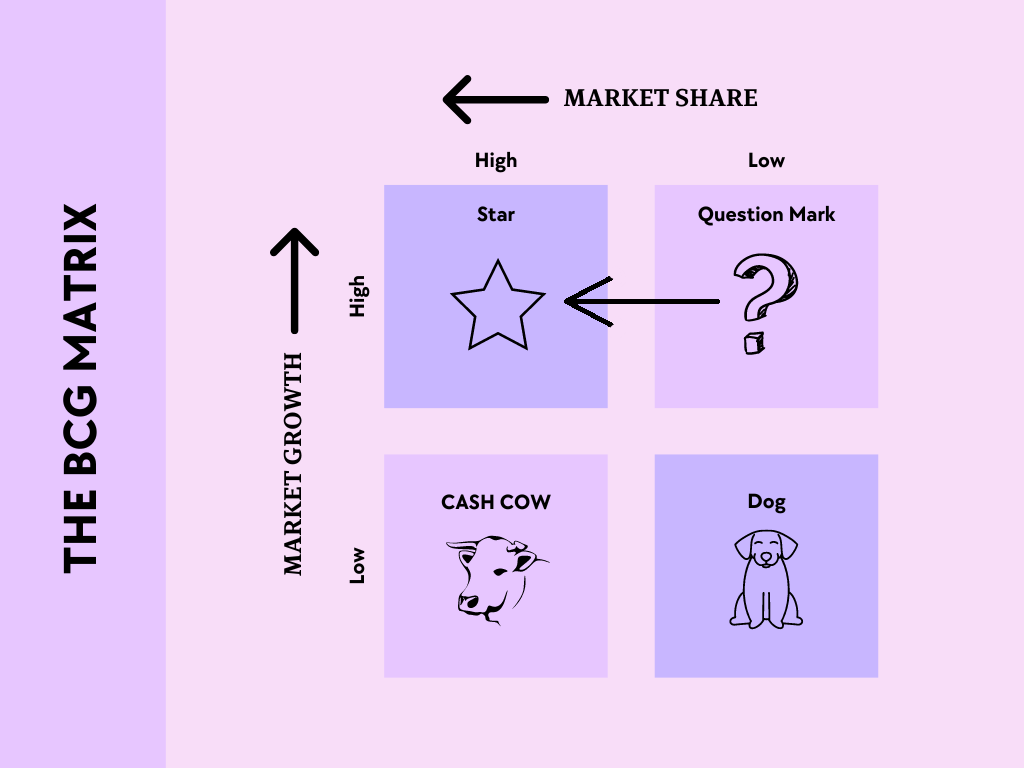
\includegraphics[width=.85\textwidth]{images/bcg_matrix.png}
\end{center}


\subsection{Analisi SWOT}
\begin{center}
    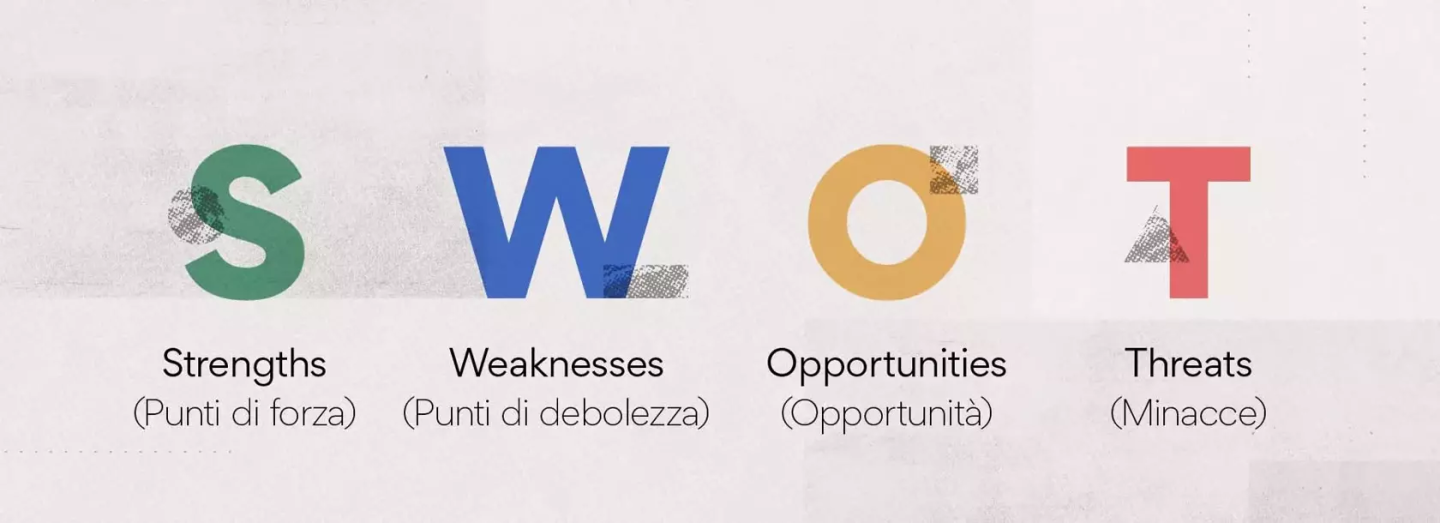
\includegraphics[width=\textwidth]{images/swot.png}
\end{center}
\subsubsection*{Punti di Forza (Strengths)}
\begin{enumerate}
    \item \textbf{Vasta selezione di vini}: Vinovo ha un catalogo ampio e diversificato di vini provenienti da diverse regioni vinicole. Questo permette all'azienda di soddisfare le preferenze dei clienti e offrire una vasta scelta di prodotti.
          % \item \textbf{Competenza nel settore del vino}: Il team di Vinovo è composto da esperti nel settore del vino con una profonda conoscenza delle varietà di uve, delle tecniche di produzione e delle tendenze del mercato. Questa competenza consente all'azienda di selezionare vini di alta qualità e di fornire consulenza esperta ai clienti.
    \item \textbf{Collaborazioni con produttori di vino}: Vinovo intende stabilire relazioni solide con produttori di vino reputati. Queste collaborazioni consentono all'azienda di ottenere vini esclusivi, introdurre nuove etichette sul mercato e garantire l'autenticità e la qualità dei prodotti offerti.
    \item \textbf{User experience digitale}: Vinovo ha sviluppato una piattaforma di e-commerce intuitiva e user-friendly. L'interfaccia di facile utilizzo, le descrizioni dettagliate dei prodotti, le recensioni dei clienti e le opzioni di ricerca avanzata migliorano l'esperienza di acquisto online dei clienti.
    \item \textbf{Servizio clienti personalizzato}: Vinovo punta ad offrire un servizio clienti di qualità, fornendo assistenza personalizzata, rispondendo prontamente alle domande e aiutando i clienti a trovare i vini più adatti alle loro preferenze.
\end{enumerate}

\subsubsection*{Punti di Debolezza (Weaknesses)}
\begin{enumerate}
    \item \textbf{Consapevolezza del marchio}: Vinovo potrebbe avere una minore consapevolezza del marchio rispetto a concorrenti più consolidati nel settore dell'e-commerce del vino. Ciò richiede sforzi continui per promuovere il marchio attraverso campagne di marketing, pubblicità mirata e collaborazioni strategiche.
    \item \textbf{Dipendenza dalla logistica}: Vinovo dipende da partner di logistica per la gestione delle consegne dei prodotti. Questa dipendenza potrebbe comportare sfide in termini di tempi di consegna, costi e gestione delle eventuali problematiche logistiche.
\end{enumerate}

\subsubsection*{Opportunità (Opportunities)}
\begin{enumerate}
    \item \textbf{Crescita del mercato dell'e-commerce del vino}: Il settore dell'e-commerce del vino è in crescita costante, offrendo opportunità di espansione per Vinovo. La comodità dell'acquisto online e la crescente preferenza dei consumatori per l'acquisto di vino online aprono nuove possibilità di business.
    \item \textbf{Esplorazione di nuovi mercati}: Vinovo può esplorare l'espansione in nuovi mercati geografici, sia a livello nazionale che internazionale nel futuro. A tal fine si può adattare l'offerta di vini per soddisfare le preferenze specifiche di queste nuove aree e ampliare la base di clienti.
    \item \textbf{Programmi di fidelizzazione dei clienti}: Si intende sviluppare programmi di fedeltà per premiare e incentivare i clienti fedeli. Ciò può contribuire a creare una base di clienti affezionati e a generare ricavi ripetuti nel lungo termine.
\end{enumerate}

\subsubsection*{Minacce (Threats)}
\begin{enumerate}
    \item \textbf{Concorrenza diretta}: Il settore dell'e-commerce del vino è altamente competitivo, con la presenza di numerosi rivenditori online e grandi attori del settore. La concorrenza può comportare una maggiore pressione sui prezzi, rendendo importante per Vinovo distinguersi attraverso la qualità dei prodotti, l'esperienza del cliente e l'innovazione continua.
    \item \textbf{Regolamentazioni e restrizioni}: Vinovo deve affrontare le regolamentazioni legate alla vendita di alcolici online, come l'età legale per l'acquisto di alcol e le norme sulla spedizione di bevande alcoliche. È importante rispettare tali norme e adottare misure per garantire la conformità.
\end{enumerate}\bigskip
In sintesi, per massimizzare le opportunità e affrontare le minacce, Vinovo può concentrarsi sulla promozione del marchio, espandere la presenza geografica per raggiungere nuovi mercati, migliorare l'efficienza logistica per garantire consegne tempestive e implementare programmi di fidelizzazione dei clienti per aumentare la fedeltà e il valore a vita del cliente. Inoltre, bisognerebbe monitorare attentamente il mercato e le tendenze del settore, adattando la sua offerta e strategia di business di conseguenza.
\newpage

\section{Team}
In questa sezione vengono descritti i membri del team imprenditoriale, evidenziando le loro esperienze, competenze, background e le posizioni che ricoprono all'interno dell'azienda. Vengono inoltre illustrate la struttura societaria e l'organigramma aziendale.

\subsection{Profili professionali e ruolo dei soggetti proponenti}
\begin{tabular}{|l|l|l|}
    \hline
    \rowcolor[HTML]{CBCEFB}
    \textbf{Nome}     & \textbf{Principali competenze}                                                                                  & \textbf{\begin{tabular}[c]{@{}l@{}}Ruolo ricoperto\\ all'interno dell'azienda\end{tabular}} \\ \hline
    Lorenzo Sequino   & \begin{tabular}[c]{@{}l@{}}Ambizione, sacrificio,\\ attitudine alla leadership\end{tabular}                     & CEO e fondatore                                                                             \\ \hline
    Roberto Ingenito  & Competenze comunicative                                                                                         & Chief Marketing Officer (CMO)                                                               \\ \hline
    Simone Ingenito   & \begin{tabular}[c]{@{}l@{}}Capacità di progettazione\\ e realizzazione\\ di interfacce e contenuti\end{tabular} & Chief UI \& UX Designer                                                                     \\ \hline
    Vincenzo Di Nardo & \begin{tabular}[c]{@{}l@{}}Conoscenze delle tecnologie\\ e degli strumenti \\ digitali moderni\end{tabular}     & Chief Technology Officer (CTO)                                                              \\ \hline
    Filippo Minieri   & \begin{tabular}[c]{@{}l@{}}Conoscenza approfondita\\ del mercato e delle \\ sue fluttuazioni\end{tabular}       & Chief Financial Officer (CFO)                                                               \\ \hline
\end{tabular}
\newpage

\subsection{Brevi curriculum dei soci}
\subsubsection*{Lorenzo Sequino - CEO e fondatore}
Laureato in Economia.\\
Esperienza pluriennale nel settore della vendita di prodotti enogastronomici.\\
Ha lavorato come responsabile delle vendite presso una nota azienda del settore.\\
Competenze imprenditoriali e conoscenza approfondita del mercato vinicolo.

\subsubsection*{Roberto Ingenito - Chief Marketing Officer (CMO)}
Laureato in Marketing.\\
Ha ricoperto il ruolo di responsabile marketing in diverse aziende, con focus sul settore del food e del vino.\\
Esperienza nell'ideazione e nell'esecuzione di strategie di marketing innovative.\\
Conoscenza approfondita delle dinamiche dei social media e delle strategie di promozione online.

\subsubsection*{Simone Ingenito - Chief UI \& UX Designer}
Laureato in Economia e Finanza.\\
Ha lavorato come consulente finanziario presso un importante studio di consulenza.\\
Esperienza nella gestione finanziaria e nel controllo di gestione.\\
Competenze solide in analisi finanziaria e pianificazione aziendale.

\subsubsection*{Vincenzo Di Nardo - Chief Technology Officer (CTO)}
Laureato in Logistica e Gestione della Supply Chain.\\
Ha lavorato come responsabile logistica presso un'azienda di distribuzione alimentare.\\
Esperienza nella gestione delle operazioni di approvvigionamento e logistica.\\
Conoscenza approfondita delle pratiche di gestione della supply chain nel settore enogastronomico.

\subsubsection*{Filippo Minieri - Chief Financial Officer (CFO)}
Laureato in Commercio Internazionale.\\
Ha una vasta esperienza nel settore delle vendite, sia in aziende nazionali che internazionali.\\
Competenze nel sviluppo di strategie di vendita efficaci e nell'acquisizione di nuovi clienti.\\
Conoscenza approfondita dei mercati esteri nel settore vinicolo.

\subsection{Assetto societario}
La forma giuridica che abbiamo scelto di adottare per la nostra startup Vinovo è la Società a Responsabilità Limitata (S.R.L.). Abbiamo optato per questa forma legale perché consente ai soci di non essere personalmente responsabili dei debiti dell'azienda e, in caso di insolvenza, la società può dichiarare fallimento senza coinvolgere i soci.\meskip
Per costituire l'impresa, abbiamo seguito le seguenti procedure conformemente alla legge:
\begin{itemize}
    \item Abbiamo redatto un atto notarile.
    \item Abbiamo pagato l'imposta di registro per l'atto costitutivo.
    \item Abbiamo versato il diritto camerale.
    \item Prima della costituzione, abbiamo pagato la tassa per la vidimazione annuale dei libri sociali.
    \item Abbiamo acquistato la vidimazione e la bollatura dei libri sociali obbligatori.
\end{itemize}
La sede legale della nostra impresa si trova presso l'ufficio dei soci in Via Vicinale Cupa Cintia 26, 80126 Napoli NA. Il Capitale Sociale è di 100.000 euro. Tutti i soci sono indicati come amministratori e le quote dell'azienda sono state equamente distribuite tra di loro, contribuendo al capitale sociale con lo stesso peso.

\section{Pianificazione operativa}
In questo capitolo, definiamo vari aspetti della pianificazione operativa per la nostra startup Vinovo. Valutiamo gli aspetti tecnologici, l'organizzazione operativa per la realizzazione dei nostri servizi, la natura e l'entità degli investimenti, i diversi costi da sostenere e la stima dei ricavi previsti.

\subsection{Piano operativo e manodopera}

Nel nostro processo di lancio del marchio sul mercato, è fondamentale analizzare attentamente le attività che richiedono attenzione e pianificazione. In particolare, concentriamo la nostra attenzione sulle competenze e le figure professionali che saranno essenziali per garantire il successo dell'operazione.

\subsubsection{Piattaforma online e social network}

Vinovo si specializza nella vendita online di prodotti enogastronomici di alta qualità. Per garantire una presenza online efficace, è fondamentale progettare e implementare una piattaforma digitale all'avanguardia, composta da un sito web. Pertanto assumiamo un esperto informatico altamente qualificato che possa guidare lo sviluppo e la gestione di questa piattaforma. Il nostro obiettivo è creare un'esperienza di acquisto fluida e intuitiva per i nostri clienti, semplificando le interazioni con i fornitori e le società di consegna attraverso l'automazione dei processi.\meskip
La promozione del marchio Vinovo richiede una presenza forte e coinvolgente sui social network, che rappresentano un canale di comunicazione fondamentale per raggiungere i nostri potenziali clienti. A tal fine, abbiamo bisogno di un social media manager esperto, dotato di solide competenze nel creare strategie di marketing efficaci sui social media. Questo professionista sarà responsabile di gestire le nostre pagine aziendali sui vari social network, creare contenuti coinvolgenti, pianificare e lanciare campagne pubblicitarie mirate e gestire le interazioni con la nostra crescente base di follower. Inoltre, il social media manager avrà anche il compito di stabilire e mantenere delle relazioni significative con influencer del settore, al fine di amplificare la visibilità del marchio Vinovo e raggiungere un pubblico più vasto.\meskip
Attraverso una solida presenza online e una strategia di social media ben definita, intendiamo posizionare il marchio Vinovo come punto di riferimento per gli amanti del buon vino. Siamo consapevoli dell'importanza di adattarci alle dinamiche digitali che sono in continua evoluzione, e di sfruttare appieno le opportunità offerte dai canali online e dai social media per raggiungere il nostro target di clientela in modo efficace ed efficiente.\meskip
In conclusione, l'assunzione di un esperto informatico per gestire la piattaforma online e di un social media manager per promuovere il marchio Vinovo sui social network rappresenta un passo cruciale nella nostra strategia di crescita e nel raggiungimento del successo nel settore enogastronomico online. Siamo determinati a offrire un'esperienza di acquisto unica e coinvolgente ai nostri clienti, mantenendo un forte legame con loro attraverso una presenza digitale dinamica e accattivante.

\subsubsection{Logistica e consegne}
Nella nostra start-up Vinovo, l'efficienza e la qualità del servizio logistico e di distribuzione sono un punto cardine per assicurare un'esperienza eccellente ai nostri clienti. Abbiamo stabilito partnership strategiche con corrieri affidabili per gestire le spedizioni a livello nazionale, prendendo in considerazione attentamente l'affidabilità e la convenienza economica.\meskip
Riconosciamo che alcuni dei nostri prodotti richiedono particolari accorgimenti durante il trasporto per garantire la freschezza e la qualità. Pertanto, abbiamo collaborazioni con aziende specializzate nel trasporto a temperatura controllata. Grazie a queste partnership, possiamo garantire che i prodotti sensibili alla temperatura siano gestiti correttamente durante il trasporto, mantenendoli nel range adeguato.\meskip
Per quanto riguarda l'organizzazione delle consegne, il nostro team imprenditoriale si occupa di coordinare e gestire questo processo cruciale. Sono supportati da dipendenti dedicati che gestiscono le richieste dei clienti e offrono un servizio clienti di alta qualità. Al fine di assumere tali impiegati, stiamo cercando individui con ottime capacità relazionali, organizzative e linguistiche. Inoltre, è essenziale avere competenze informatiche per gestire in modo efficiente i sistemi di gestione delle consegne e fornire supporto tecnico ai clienti, se necessario.\meskip
Siamo fermamente convinti che un'organizzazione efficace delle consegne e un servizio clienti impeccabile siano elementi chiave per il successo della nostra start-up. Ci impegniamo a creare un'esperienza di acquisto piacevole e soddisfacente per i nostri clienti, adottando tutte le misure necessarie per garantire la puntualità e l'integrità delle consegne. Siamo entusiasti di costruire un team competente e dedicato che ci aiuterà a realizzare la nostra visione di offrire prodotti enogastronomici di alta qualità, consegnati con cura e professionalità.

\subsubsection{Imballaggio dei prodotti}
Nella nostra start-up, Vinovo, diamo molto peso alla corretta distribuzione dei nostri prodotti. Per garantire la qualità dei nostri vini durante il trasporto, utilizzeremo imballaggi specifici progettati appositamente per soddisfare le esigenze delle spedizioni. Questi imballaggi includeranno una varietà di scatole di cartone con diverse forme e dimensioni, tutte contrassegnate con il nostro logo Vinovo.\meskip
L'etichettatura con il nostro logo distintivo non solo contribuirà a promuovere la nostra marca, ma faciliterà anche il monitoraggio e la tracciabilità dei nostri prodotti lungo l'intera catena di distribuzione. \meskip
Per gestire in modo efficiente gli imballaggi e garantire uno stoccaggio adeguato, avremo bisogno di uno spazio di magazzino appositamente dedicato. Un magazziniere altamente qualificato e attento sarà responsabile della gestione, dell'organizzazione e del controllo degli imballaggi nel nostro magazzino. Sarà la figura chiave che si assicurerà che gli imballaggi siano correttamente immagazzinati, pronti per le spedizioni e in condizioni ottimali per garantire la freschezza dei nostri prodotti.\meskip
Inoltre, per garantire la qualità dei nostri prodotti, collaboreremo strettamente con i nostri fornitori. Abbiamo stabilito un'ottima relazione con loro e ci assicuriamo che gli imballaggi siano gestiti nel modo corretto, rispettando le specifiche richieste dalla nostra azienda. I fornitori saranno responsabili dell'imballaggio accurato dei nostri prodotti, utilizzando materiali appropriati e seguendo scrupolosamente le linee guida che abbiamo fornito loro.\meskip
La nostra attenzione ai dettagli e l'impegno per garantire la qualità dei nostri prodotti si estendono anche all'imballaggio e alla logistica. Siamo determinati a offrire una presentazione impeccabile e una distribuzione efficiente dei nostri vini, riconoscendo l'importanza di un imballaggio adeguato per preservare la loro integrità durante il trasporto.

\begin{center}
    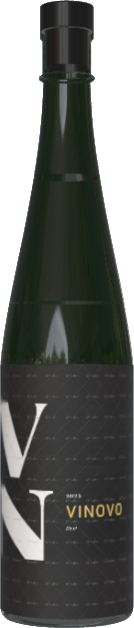
\includegraphics[height=.5\textwidth]{images/bottiglia nera.png}
    \quad
    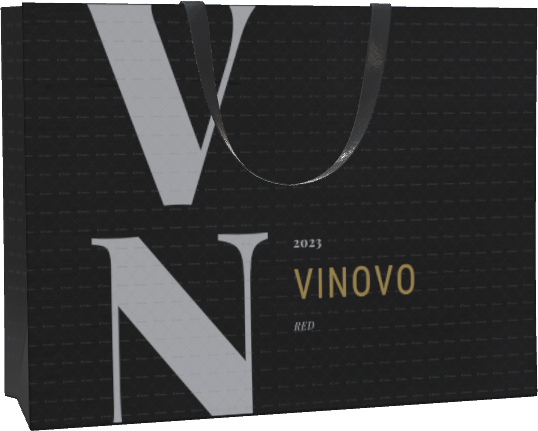
\includegraphics[height=.5\textwidth]{images/busta nera.png}
\end{center}
\begin{center}
    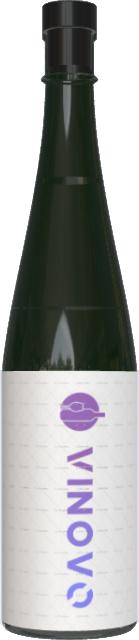
\includegraphics[height=.5\textwidth]{images/bottiglia bianca.png}
    \quad
    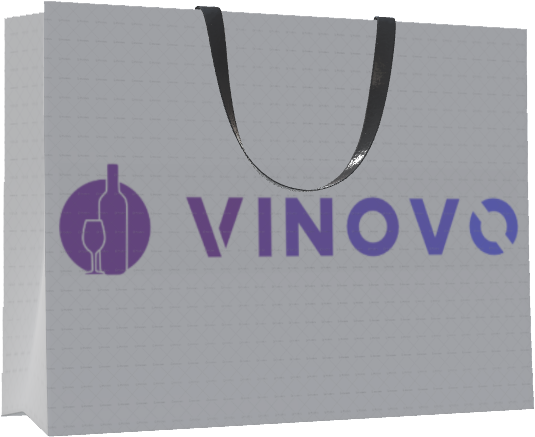
\includegraphics[height=.5\textwidth]{images/busta bianca.png}
\end{center}

\subsubsection{Magazzino}
Abbiamo identificato magazzini ideali per la nostra start up che ci permettono un facile accesso alle principali vie di trasporto.
Prestiamo molta attenzione all'organizzazione del magazzino. Sarà suddiviso in aree specifiche per la conservazione e la gestione dei prodotti, ottimizzando gli spazi per massimizzare l'efficienza delle operazioni di stoccaggio e preparazione delle spedizioni. Utilizzeremo scaffalature robuste e sistemi di archiviazione appropriati per garantire che i prodotti siano posizionati in modo sicuro e accessibile.
L'attenzione dedicata all'organizzazione riflette l'impegno e la cura che mettiamo in ogni aspetto del nostro business.

\subsubsection{Rapporti con i fornitori e controllo di qualità}
Data la vasta gamma di prodotti che offriremo nella nostra start-up Vinovo, la gestione di una rete complessa di rapporti con i fornitori su tutto il territorio nazionale sarà di fondamentale importanza. Al fine di garantire la qualità dei nostri prodotti e mantenere relazioni solide con i fornitori, stiamo facendo piani per assumere dipendenti altamente qualificati che si occuperanno di individuare nuovi potenziali fornitori e monitorare costantemente la qualità dei prodotti offerti.\meskip
Poiché i nostri fornitori potrebbero essere distribuiti in diverse regioni d'Italia, la disponibilità a spostarsi autonomamente sarà un requisito essenziale per questi dipendenti.
Essi avranno il compito di visitare regolarmente i nostri partner per verificare personalmente le pratiche agricole, il processo di produzione e la conformità ai nostri standard qualitativi. Saranno responsabili di valutare attentamente la sostenibilità ambientale, l'etica aziendale e la sicurezza alimentare dei nostri fornitori. Inoltre, saranno in grado di fornire una consulenza tecnica sulle caratteristiche nutrizionali e sulle scienze agrarie dei prodotti.
La capacità di gestire viaggi di lavoro e organizzare le visite in modo efficiente saranno competenze altamente apprezzate.\meskip
Per ricoprire tali ruoli, cercheremo dipendenti con competenze specifiche nel campo nutrizionale o delle scienze agrarie. La conoscenza di questi settori sarà fondamentale per valutare l'origine dei prodotti, l'uso di additivi o trattamenti e la qualità nutrizionale degli alimenti. Saranno inoltre richieste buone capacità relazionali per gestire con successo le interazioni con i fornitori e negoziare accordi favorevoli per la nostra azienda.\meskip
Riteniamo che l'attenzione alla qualità dei nostri prodotti e alle relazioni con i fornitori sia di primaria importanza per il successo della nostra start-up. L'assunzione di dipendenti qualificati con competenze specializzate ci permetterà di mantenere un controllo costante sulla qualità dei nostri prodotti e di sviluppare relazioni di fiducia con i nostri fornitori. Siamo determinati a offrire ai nostri clienti una selezione di vini di alta qualità provenienti da fornitori affidabili e responsabili, e siamo entusiasti di costruire un team competente che realizzerà questa visione.

\subsubsection{ERP e gestione dell'azienda}
Data la complessità della nostra catena di approvvigionamento, abbiamo implementato un sistema digitale avanzato per ottimizzare e gestire in modo efficiente i nostri processi logistici. Per fare ciò, ci avvaliamo di un potente software di Enterprise Resource Planning (ERP) che ci consente di integrare e implementare tutti i processi rilevanti per il nostro business.\meskip
L'ERP che abbiamo scelto è stato selezionato dopo un'attenta valutazione di diverse offerte di soluzioni, prendendo in considerazione le diverse caratteristiche e i costi associati. Il software ERP che abbiamo adottato si adatta perfettamente alle nostre esigenze e ci offre funzionalità avanzate per la gestione delle scorte, l'inventario, il monitoraggio delle spedizioni e molto altro ancora. Questo sistema digitale ci consente di avere una visione completa e in tempo reale di tutte le attività legate alla logistica e alla distribuzione dei nostri prodotti.\meskip
Inizialmente, il nostro team imprenditoriale è stato formato sull'utilizzo di questo software ERP, al fine di garantire una corretta implementazione e una gestione efficace dei processi logistici. Abbiamo fornito loro una formazione approfondita sulle funzionalità del software e sulle procedure operative correlate. Nel corso dei prossimi anni, estenderemo l'accesso al software anche ad altri dipendenti chiave che hanno seguito un corso di formazione specifico, al fine di coinvolgere un numero sempre maggiore di persone nella gestione ottimizzata dei processi logistici.\meskip
Attraverso l'implementazione di questo sistema digitale avanzato, siamo fiduciosi che saremo in grado di garantire un avvio e un funzionamento efficiente della nostra start-up. L'automazione dei processi logistici, la tracciabilità delle merci e la gestione ottimizzata delle scorte ci permetteranno di offrire un servizio di alta qualità ai nostri clienti e di mantenere un controllo rigoroso sulla nostra catena di approvvigionamento. Siamo entusiasti di sfruttare al massimo questa tecnologia all'avanguardia per garantire il successo della nostra start-up.

\subsection{Stima del prezzo di vendita / acquisto}
La stima dei ricavi e dei costi è un processo complesso poiché il valore del vino può variare in base alla sua qualità, anche se rientra nella stessa categoria di prodotto. Pertanto, è necessario determinare un prezzo medio di vendita e di acquisto dei prodotti. Per affrontare questa sfida, è stato adottato il seguente metodo:
\begin{enumerate}
    \item È stata effettuata una selezione dei prodotti più noti a livello nazionale e che hanno suscitato maggiore interesse tra i consumatori.
    \item Si presume che i prodotti elencati siano rappresentativi di tutte le vendite e gli acquisti effettuati. Pertanto, per calcolare i ricavi e i costi di acquisto dei prodotti, viene utilizzato il prezzo medio.
\end{enumerate}
È importante sottolineare che sebbene possano esserci variazioni nei prezzi e nelle quantità per altri prodotti non elencati, si ritiene che l'uso di prodotti noti e popolari offra una stima ragionevole dei ricavi e dei costi complessivi.\meskip
Dalla seguente tabella, si ottengono i seguenti prezzi medi:
\begin{center}
    Prezzo di vendita medio: $12,23$€\\
    Prezzo di acquisto medio: $7,09$€
\end{center}
\begin{longtable}{@{}|l|l|c|c|}
    \hline
    \rowcolor[HTML]{CBCEFB}
    Regione              & Prodotto                                                                  & \begin{tabular}[c]{@{}c@{}}Prezzo di\\ Vendita (€)\end{tabular} & \multicolumn{1}{l|}{\cellcolor[HTML]{CBCEFB}\begin{tabular}[c]{@{}l@{}}Prezzo di\\ acquisto (€)\end{tabular}} \\ \hline
    Abruzzo              & Montepulciano d'Abruzzo                                                   & 9,90 €                                                          & 5,74€                                                                                                         \\ \hline
                         & Trebbiano d'Abruzzo                                                       & 15,00 €                                                         & 8,70€                                                                                                         \\ \hline
                         & Pecorino                                                                  & 8,90 €                                                          & 5,16€                                                                                                         \\ \hline
                         & Cerasuolo d'Abruzzo                                                       & 13,90 €                                                         & 8,06€                                                                                                         \\ \hline
    Basilicata           & Aglianico del Vulture                                                     & 10,00 €                                                         & 5,80€                                                                                                         \\ \hline
                         & Matera                                                                    & 12,90 €                                                         & 7,48€                                                                                                         \\ \hline
                         & Terre dell'Alta Val d'Agri                                                & 8,90 €                                                          & 5,16€                                                                                                         \\ \hline
                         & Grottino di Roccanova                                                     & 9,90 €                                                          & 5,74€                                                                                                         \\ \hline
    Campania             & Aglianico del Vulture                                                     & 13,90 €                                                         & 8,06€                                                                                                         \\ \hline
                         & Fiano di Avellino                                                         & 10,00 €                                                         & 5,80€                                                                                                         \\ \hline
                         & Greco di Tufo                                                             & 12,90 €                                                         & 7,48€                                                                                                         \\ \hline
                         & Taurasi                                                                   & 8,90 €                                                          & 5,16€                                                                                                         \\ \hline
    Emilia Romagna       & Lambrusco                                                                 & 13,90 €                                                         & 8,06€                                                                                                         \\ \hline
                         & Sangiovese di Romagna                                                     & 11,90 €                                                         & 6,90€                                                                                                         \\ \hline
                         & Albana di Romagna                                                         & 10,00 €                                                         & 5,80€                                                                                                         \\ \hline
                         & Pignoletto                                                                & 13,90 €                                                         & 8,06€                                                                                                         \\ \hline
    Fruli Venezia Giulia &                                                                           & 15,00 €                                                         & 8,70€                                                                                                         \\ \hline
                         & Friulano                                                                  & 8,90 €                                                          & 5,16€                                                                                                         \\ \hline
                         & Pinot Bianco                                                              & 13,90 €                                                         & 8,06€                                                                                                         \\ \hline
                         & Ribolla Gialla                                                            & 11,90 €                                                         & 6,90€                                                                                                         \\ \hline
                         & Sauvignon Blanc                                                           & 13,90 €                                                         & 8,06€                                                                                                         \\ \hline
    Lazio                & Frascati                                                                  & 8,90 €                                                          & 5,16€                                                                                                         \\ \hline
                         & Cesanese del Piglio                                                       & 13,90 €                                                         & 8,06€                                                                                                         \\ \hline
                         & Aleatico di Gradoli                                                       & 13,90 €                                                         & 8,06€                                                                                                         \\ \hline
                         & Marino                                                                    & 11,90 €                                                         & 6,90€                                                                                                         \\ \hline
    Liguria              & Cinque Terre                                                              & 13,90 €                                                         & 8,06€                                                                                                         \\ \hline
                         & Pigato                                                                    & 8,90 €                                                          & 5,16€                                                                                                         \\ \hline
                         & Vermentino di Liguria                                                     & 13,90 €                                                         & 8,06€                                                                                                         \\ \hline
                         & Rossese di Dolceacqua                                                     & 13,90 €                                                         & 8,06€                                                                                                         \\ \hline
    Piemonte             & Barolo                                                                    & 15,00 €                                                         & 8,70€                                                                                                         \\ \hline
                         & Barbaresco                                                                & 13,90 €                                                         & 8,06€                                                                                                         \\ \hline
                         & Barbera d'Asti                                                            & 10,00 €                                                         & 5,80€                                                                                                         \\ \hline
                         & Gavi                                                                      & 12,90 €                                                         & 7,48€                                                                                                         \\ \hline
    Sicilia              & Nero d'Avola                                                              & 8,90 €                                                          & 5,16€                                                                                                         \\ \hline
                         & Etna Rosso                                                                & 13,90 €                                                         & 8,06€                                                                                                         \\ \hline
                         & Marsala                                                                   & 11,90 €                                                         & 6,90€                                                                                                         \\ \hline
                         & Moscato di Pantelleria                                                    & 10,00 €                                                         & 5,80€                                                                                                         \\ \hline
    Umbria               & Sagrantino di Montefalco                                                  & 13,90 €                                                         & 8,06€                                                                                                         \\ \hline
                         & Orvieto                                                                   & 15,00 €                                                         & 8,70€                                                                                                         \\ \hline
                         & Torgiano Rosso Riserva                                                    & 8,90 €                                                          & 5,16€                                                                                                         \\ \hline
                         & Grechetto                                                                 & 13,90 €                                                         & 8,06€                                                                                                         \\ \hline
    Marche               & \begin{tabular}[c]{@{}l@{}}Verdicchio dei\\ Castelli di Jesi\end{tabular} & 11,90 €                                                         & 6,90€                                                                                                         \\ \hline
                         & Rosso Conero                                                              & 13,90 €                                                         & 8,06€                                                                                                         \\ \hline
                         & Lacrima di Morro d'Alba                                                   & 8,90 €                                                          & 5,16€                                                                                                         \\ \hline
                         & Vernaccia di Serrapetrona                                                 & 13,90 €                                                         & 8,06€                                                                                                         \\ \hline
    Puglia               & Primitivo di Manduria                                                     & 13,90 €                                                         & 8,06€                                                                                                         \\ \hline
                         & Salice Salentino                                                          & 11,90 €                                                         & 6,90€                                                                                                         \\ \hline
                         & Negroamaro                                                                & 13,90 €                                                         & 8,06€                                                                                                         \\ \hline
                         & Castel del Monte                                                          & 8,90 €                                                          & 5,16€                                                                                                         \\ \hline
    Sardegna             & Cannonau di Sardegna                                                      & 13,90 €                                                         & 8,06€                                                                                                         \\ \hline
                         & Vermentino di Gallura                                                     & 13,90 €                                                         & 8,06€                                                                                                         \\ \hline
                         & Carignano del Sulcis                                                      & 15,00 €                                                         & 8,70€                                                                                                         \\ \hline
                         & Nuragus di Cagliari                                                       & 13,90 €                                                         & 8,06€                                                                                                         \\ \hline
    Sicilia              & Nero d'Avola                                                              & 10,00 €                                                         & 5,80€                                                                                                         \\ \hline
                         & Etna Rosso                                                                & 12,90 €                                                         & 7,48€                                                                                                         \\ \hline
                         & Marsala                                                                   & 8,90 €                                                          & 5,16€                                                                                                         \\ \hline
                         & Moscato di Pantelleria                                                    & 13,90 €                                                         & 8,06€                                                                                                         \\ \hline
    Calabria             & Cirò                                                                      & 11,90 €                                                         & 6,90€                                                                                                         \\ \hline
                         & Greco di Bianco                                                           & 10,00 €                                                         & 5,80€                                                                                                         \\ \hline
                         & Gaglioppo                                                                 & 13,90 €                                                         & 8,06€                                                                                                         \\ \hline
                         & Magliocco                                                                 & 15,00 €                                                         & 8,70€                                                                                                         \\ \hline
    Valle d'Aosta        & \begin{tabular}[c]{@{}l@{}}Blanc de Morgex\\ et de La Salle\end{tabular}  & 8,90 €                                                          & 5,16€                                                                                                         \\ \hline
                         & Torrette                                                                  & 13,90 €                                                         & 8,06€                                                                                                         \\ \hline
                         & Petite Arvine                                                             & 11,90 €                                                         & 6,90€                                                                                                         \\ \hline
                         & Fumin                                                                     & 13,90 €                                                         & 8,06€                                                                                                         \\ \hline
    Molise               & Tintilia del Molise                                                       & 8,90 €                                                          & 5,16€                                                                                                         \\ \hline
                         & Biferno                                                                   & 13,90 €                                                         & 8,06€                                                                                                         \\ \hline
                         & Falanghina del Molise                                                     & 13,90 €                                                         & 8,06€                                                                                                         \\ \hline
                         & Aglianico del Molise                                                      & 11,90 €                                                         & 6,90€                                                                                                         \\ \hline
    Lombardia            & Franciacorta                                                              & 13,90 €                                                         & 8,06€                                                                                                         \\ \hline
                         & Valtellina Superiore                                                      & 8,90 €                                                          & 5,16€                                                                                                         \\ \hline
                         & Lugana                                                                    & 13,90 €                                                         & 8,06€                                                                                                         \\ \hline
                         & Moscato di Scanzo                                                         & 13,90 €                                                         & 8,06€                                                                                                         \\ \hline
    Veneto               & Amarone della Valpolicella                                                & 15,00 €                                                         & 8,70€                                                                                                         \\ \hline
                         & Prosecco                                                                  & 13,90 €                                                         & 8,06€                                                                                                         \\ \hline
                         & Valpolicella                                                              & 10,00 €                                                         & 5,80€                                                                                                         \\ \hline
                         & Soave                                                                     & 12,90 €                                                         & 7,48€                                                                                                         \\ \hline
    Trentino-Alto Adige  & Pinot Nero                                                                & 8,90 €                                                          & 5,16€                                                                                                         \\ \hline
                         & Pinot Grigio                                                              & 13,90 €                                                         & 8,06€                                                                                                         \\ \hline
                         & Lagrein                                                                   & 11,90 €                                                         & 6,90€                                                                                                         \\ \hline
                         & Moscato Giallo                                                            & 10,00 €                                                         & 5,80€                                                                                                         \\ \hline
\end{longtable}

\subsection{Stima delle vendite e dei ricavi}
Secondo i dati riportati nell'"annual report" di Valoritalia del 2022, il settore del vino italiano ha registrato un calo del -3,8\%. Questa diminuzione può essere attribuita principalmente all'impatto negativo del conflitto russo-ucraino e alla crisi energetica, che hanno determinato un rallentamento dei flussi economici in diversi settori.\meskip
È interessante notare che il settore del vino aveva vissuto un periodo di grande successo nel 2019, con una crescita del 20\%. Tuttavia, l'anno successivo, il 2020, a causa della pandemia globale, l'economia nel suo complesso ha subito un forte colpo, e anche il settore vinicolo ne ha risentito. Solo nel 2021 si è cominciato a intravedere una ripresa.\meskip
Tuttavia, a partire da febbraio del 2022, l'escalation del conflitto russo-ucraino ha determinato una situazione ancora più difficile per il settore del vino italiano. Questo conflitto ha portato ad un clima di incertezza e speculazione economica, con una scarsità di materie prime e un aumento dell'inflazione. L'economia mondiale ha iniziato a mostrare segni di una "economia di guerra", con gravi ripercussioni su diverse industrie, compresa quella del vino.\meskip
È fondamentale considerare che l'andamento del settore vinicolo dipende da molti fattori, tra cui le condizioni economiche globali, i cambiamenti nelle abitudini dei consumatori e gli eventi geopolitici. \bskip
Secondo i dati Istat sui consumi di alcolici in Italia, nel 2021 sono quasi 30 milioni gli italiani che consumano vino:
\begin{itemize}[topsep=0pt]
    \item il 55\% della popolazione adulta italiana
    \item il 66\% tra i maschi e il 44\% tra le femmine.
\end{itemize}
Di questi 30 milioni, 8 milioni acquistano vino online.\meskip
Secondo i dati riportati da "WineNews.it", in media ogni italiano effettua 0.05 transazioni online all'anno su un e-commerc di vini, acquistando in media 6.25 prodotti per ogni transazione.\meskip
Inoltre, ipotizziamo che Vinovo conquisti lo 0.7\% del mercato nel primo anno e che tale quota tenderà a crescere di circa il 122\% l'anno (per i primi 3 anni) analizzando anche la crescita dei nostri competitors.\\
Utilizziamo questi dati per stimare e valutare il numero di vendite:
\begin{center}
    Prodotti venduti il 1° anno: $0,05 \times 6,25 \times 0,007  \times 8.000.000 = 17.500$\\
    Prodotti venduti il 2° anno: $0,05 \times 6,25 \times 0,0155 \times 8.000.000 = 38.750$\\
    Prodotti venduti il 3° anno: $0,05 \times 6,25 \times 0,0345 \times 8.000.000 = 86.250$
\end{center}
\begin{center}
    Ricavi vendita 1° anno = $17.500 \times 12,23€ = 214.025€$\\
    Ricavi vendita 2° anno = $38.750 \times 12,23€ = 473.912,5€$\\
    Ricavi vendita 3° anno = $86.250 \times 12,23€ = 1.054.837,5€$
\end{center}

\subsection{Stima dei costi}
Di seguito si riporta la tabella con i costi relativi agli stipendi dei dipendenti e con il numero di assunzioni anno per anno
\begin{longtable}{lcccc}
    \hline
    \rowcolor[HTML]{CBCEFB}
    \multicolumn{1}{|c|}{\cellcolor[HTML]{CBCEFB}\textbf{\begin{tabular}[c]{@{}c@{}}STIPENDIO\\ DIPENDENTI\end{tabular}}} & \multicolumn{1}{c|}{\cellcolor[HTML]{CBCEFB}\textbf{\begin{tabular}[c]{@{}c@{}}Numero\\ dipendenti\\ anno 1\end{tabular}}} & \multicolumn{1}{c|}{\cellcolor[HTML]{CBCEFB}\textbf{\begin{tabular}[c]{@{}c@{}}Numero\\ dipendenti\\ anno 2\end{tabular}}} & \multicolumn{1}{c|}{\cellcolor[HTML]{CBCEFB}\textbf{\begin{tabular}[c]{@{}c@{}}Numero\\ dipendenti\\ anno 3\end{tabular}}} & \multicolumn{1}{c|}{\cellcolor[HTML]{CBCEFB}\textbf{\begin{tabular}[c]{@{}c@{}}Stipendio\\ mensile\end{tabular}}} \\ \hline
    \multicolumn{1}{|l|}{Impiegato logistica}                                                                             & \multicolumn{1}{c|}{1}                                                                                                     & \multicolumn{1}{c|}{1}                                                                                                     & \multicolumn{1}{c|}{2}                                                                                                     & \multicolumn{1}{c|}{€ 1.600}                                                                                      \\ \hline
    \multicolumn{1}{|l|}{Impiegato marketing}                                                                             & \multicolumn{1}{c|}{1}                                                                                                     & \multicolumn{1}{c|}{1}                                                                                                     & \multicolumn{1}{c|}{2}                                                                                                     & \multicolumn{1}{c|}{€ 2.000}                                                                                      \\ \hline
    \multicolumn{1}{|l|}{Informatico}                                                                                     & \multicolumn{1}{c|}{1}                                                                                                     & \multicolumn{1}{c|}{1}                                                                                                     & \multicolumn{1}{c|}{1}                                                                                                     & \multicolumn{1}{c|}{€ 1.700}                                                                                      \\ \hline
    \multicolumn{1}{|l|}{Impiegato servizio clienti}                                                                      & \multicolumn{1}{c|}{2}                                                                                                     & \multicolumn{1}{c|}{3}                                                                                                     & \multicolumn{1}{c|}{4}                                                                                                     & \multicolumn{1}{c|}{€ 1.300}                                                                                      \\ \hline
    \multicolumn{1}{|l|}{Magazziniere}                                                                                    & \multicolumn{1}{c|}{0}                                                                                                     & \multicolumn{1}{c|}{1}                                                                                                     & \multicolumn{1}{c|}{2}                                                                                                     & \multicolumn{1}{c|}{€ 1.400}                                                                                      \\ \hline
    \multicolumn{1}{|l|}{\cellcolor[HTML]{CBCEFB}}                                                                        & \multicolumn{1}{c|}{\cellcolor[HTML]{CBCEFB}\textbf{Anno 1}}                                                               & \multicolumn{1}{c|}{\cellcolor[HTML]{CBCEFB}\textbf{Anno 2}}                                                               & \multicolumn{1}{c|}{\cellcolor[HTML]{CBCEFB}\textbf{Anno 3}}                                                               &                                                                                                                   \\ \cline{2-4}
    \multicolumn{1}{|l|}{\multirow{-2}{*}{\cellcolor[HTML]{CBCEFB}\textbf{Costo stipendio totale}}}                       & \multicolumn{1}{c|}{€ 98.400}                                                                                              & \multicolumn{1}{c|}{€ 130.800}                                                                                             & \multicolumn{1}{c|}{€ 210.000}                                                                                             &                                                                                                                   \\ \cline{1-4}
\end{longtable}
\begin{itemize}
    \item Impiegato logistica: si occupa della pianificazione e dell'organizzazione delle spedizioni di merci
    \item Impiegato marketing: si occupa di sviluppare e implementare strategie di marketing al fine di promuovere i prodotti o i servizi della startup
    \item Informatico: si occupa dello sviluppo e del mantenimento del sito web
    \item Impiegato servizi clienti: si occupa di fornire assistenza e supporto ai clienti
    \item Magazziniere: si occupa della gestione delle operazioni all'interno del magazzino
\end{itemize}\newpage
\begin{longtable}{|lccc|}
    \hline
    \multicolumn{4}{|l|}{\cellcolor[HTML]{CBCEFB}\textbf{PRODUZIONE VINOVO (costo medio per bottiglia)}}                           \\ \hline
    \multicolumn{1}{|l|}{}                                  & \multicolumn{1}{c|}{Anno 1} & \multicolumn{1}{c|}{Anno 2} & € Anno 3 \\ \hline
    \multicolumn{1}{|l|}{Costo produzione di una bottiglia} & \multicolumn{1}{c|}{€ 5}    & \multicolumn{1}{c|}{€ 5}    & € 5      \\ \hline
    \multicolumn{1}{|l|}{Imbottigliamento}                  & \multicolumn{1}{c|}{€ 0,30} & \multicolumn{1}{c|}{€ 0,26} & € 0,25   \\ \hline
    \multicolumn{1}{|l|}{Etichetta personalizzata Vinovo}   & \multicolumn{1}{c|}{€ 0,02} & \multicolumn{1}{c|}{€ 0,02} & € 0,02   \\ \hline
    \multicolumn{1}{|l|}{Imballaggio}                       & \multicolumn{1}{c|}{€ 1,20} & \multicolumn{1}{c|}{€ 1,10} & € 1,00   \\\hline
\end{longtable}
\begin{itemize}
    \item Costo produzione di una bottiglia: comprende il costo della produzione del vino e della bottiglia vuota
    \item Imbottigliamento: processo di confezionamento del vino in bottiglie incluso pulizia, riempimento e tappatura
    \item Etichetta personalizzata Vinovo: costo delle etichette acquistate in bundle da fornitori esterni
    \item Imballagio: comprende il costo del singolo scatolo e dei materiali utilizzati per proteggere le bottiglie
\end{itemize}
\begin{longtable}{|lccc|}
    \hline
    \rowcolor[HTML]{CBCEFB}
    \multicolumn{1}{|l|}{\cellcolor[HTML]{CBCEFB}\textbf{COSTO GESTIONE}}                                                                                 & \multicolumn{1}{c|}{\cellcolor[HTML]{CBCEFB}\textbf{Anno 1}}   & \multicolumn{1}{c|}{\cellcolor[HTML]{CBCEFB}\textbf{Anno 2}}   & \textbf{Anno 3}   \\ \hline
    \multicolumn{4}{|l|}{\textbf{CANTINA}}                                                                                                                                                                                                                                                                      \\ \hline
    \multicolumn{1}{|l|}{Affitto}                                                                                                                         & \multicolumn{1}{c|}{€ 7.800}                                   & \multicolumn{1}{c|}{€ 7.800}                                   & € 10.000          \\ \hline
    \multicolumn{1}{|l|}{Utenze}                                                                                                                          & \multicolumn{1}{c|}{€ 800}                                     & \multicolumn{1}{c|}{€ 830}                                     & € 980             \\ \hline
    \multicolumn{1}{|l|}{Pulizia e manutenzione}                                                                                                          & \multicolumn{1}{c|}{€ 1.000}                                   & \multicolumn{1}{c|}{€ 1.000}                                   & € 1.200           \\ \hline
    \multicolumn{4}{|l|}{\textbf{INFRASTRUTTURE}}                                                                                                                                                                                                                                                               \\ \hline
    \multicolumn{1}{|l|}{Sviluppo sito web}                                                                                                               & \multicolumn{1}{c|}{€ 6.500}                                   & \multicolumn{1}{c|}{€ 2.100}                                   & € 2.100           \\ \hline
    \multicolumn{1}{|l|}{Database clientela}                                                                                                              & \multicolumn{1}{c|}{€ 1.100}                                   & \multicolumn{1}{c|}{€ 1.600}                                   & € 2.000           \\ \hline
    \multicolumn{1}{|l|}{ERP}                                                                                                                             & \multicolumn{1}{c|}{€ 5.500}                                   & \multicolumn{1}{c|}{€ 5.500}                                   & € 5.500           \\ \hline
    \multicolumn{4}{|l|}{\textbf{MARKETING}}                                                                                                                                                                                                                                                                    \\ \hline
    \multicolumn{1}{|l|}{Pubblicità online}                                                                                                               & \multicolumn{1}{c|}{€ 800}                                     & \multicolumn{1}{c|}{€ 1.200}                                   & € 1.500           \\ \hline
    \multicolumn{1}{|l|}{Content creation}                                                                                                                & \multicolumn{1}{c|}{€ 600}                                     & \multicolumn{1}{c|}{€ 800}                                     & € 1.100           \\ \hline
    \multicolumn{1}{|l|}{Collaborazione ed eventi}                                                                                                        & \multicolumn{1}{c|}{€ 12.000}                                  & \multicolumn{1}{c|}{€ 15.000}                                  & € 20.000          \\ \hline
    \multicolumn{1}{|l|}{Produzione oggetti brand "Vinovo"}                                                                                               & \multicolumn{1}{c|}{€ 5.000}                                   & \multicolumn{1}{c|}{€ 6.500}                                   & € 8.000           \\ \hline
    \multicolumn{4}{|l|}{\textbf{RICERCA E SVILUPPO}}                                                                                                                                                                                                                                                           \\ \hline
    \multicolumn{1}{|l|}{Test qualità del vino "Vinovo"}                                                                                                  & \multicolumn{1}{c|}{€ 1.700}                                   & \multicolumn{1}{c|}{€ 2.000}                                   & € 2.500           \\ \hline
    \multicolumn{4}{|l|}{\textbf{ALTRO}}                                                                                                                                                                                                                                                                        \\ \hline
    \multicolumn{1}{|l|}{Costo S.R.L.}                                                                                                                    & \multicolumn{1}{c|}{€ 600}                                     & \multicolumn{1}{c|}{€ 600}                                     & € 600             \\ \hline
    \rowcolor[HTML]{CBCEFB}
    \multicolumn{1}{|l|}{\cellcolor[HTML]{CBCEFB}\textbf{\begin{tabular}[c]{@{}l@{}}COSTO TOTALE GESTIONE\\ (produzione bottiglie escluse)\end{tabular}}} & \multicolumn{1}{c|}{\cellcolor[HTML]{CBCEFB}\textbf{€ 43.407}} & \multicolumn{1}{c|}{\cellcolor[HTML]{CBCEFB}\textbf{€ 44.930}} & \textbf{€ 55.480} \\ \hline
\end{longtable}
\begin{itemize}
    \item Sviluppo sito web: durante il primo anno, lo sviluppo iniziale del sito comporta costi più elevati in quanto viene creato da zero. Negli anni successivi, invece, si verificano solo aggiornamenti periodici.
    \item Database clientela: il costo del database tende ad aumentare nel corso degli anni in quanto la quantità di dati immagazzinati cresce.
\end{itemize}


\subsection{Piano investimenti}
Per avviare l'attività imprenditoriale, sono necessari alcuni investimenti iniziali, riportati di seguito insieme alle relative spese e alla loro quota di ammortamento.\meskip
\begin{tabular}{|l|l|c}
    \hline
    \rowcolor[HTML]{CBCEFB}
    Investimento                                                                                 & Prezzo                          & \multicolumn{1}{c|}{\cellcolor[HTML]{CBCEFB}Ammortamento} \\ \hline
    \begin{tabular}[c]{@{}l@{}}Strumentazione per la produzione\\ del vino "Vinovo"\end{tabular} & 60.000€                         & \multicolumn{1}{c|}{15\%}                                 \\ \hline
    Terreno agricolo (10mila  mq)                                                                & 30.000€                         & \multicolumn{1}{c|}{20\%}                                 \\ \hline
    Prodotti agricoli                                                                            & 1000€                           & \multicolumn{1}{c|}{50\%}                                 \\ \hline
    Scaffali magazzino                                                                           & 2500€                           & \multicolumn{1}{c|}{25\%}                                 \\ \hline
    Marketing                                                                                    & 8000€                           & \multicolumn{1}{c|}{20\%}                                 \\ \hline
    \cellcolor[HTML]{CBCEFB}Totale                                                               & \cellcolor[HTML]{CBCEFB}101500€ & \multicolumn{1}{l}{}                                      \\ \cline{1-2}
\end{tabular}
\begin{itemize}
    \item Strumentazione per la produzione del vino "Vinovo":
    \item Terreno agricolo (10mila mq): la qualità del terreno è un elemento fondamentale per la produzione del nostro vino. Per garantire la migliore qualità possibile, abbiamo investito nell'acquisto di un terreno di elevata qualità. Inoltre, siamo fortunati ad aver ereditato altri 2 ettari di terreno, che ci consentono di ampliare la nostra produzione.
    \item Prodotti agricoli: include prodotti come fertilizzanti
    \item Marketing: il nostro team ha deciso di affidarsi a un'agenzia pubblicitaria specializzata in marketing e comunicazione per gestire tutti gli aspetti promozionali. L'agenzia si occuperà di realizzare un coinvolgente video promozionale, appositamente creato per essere diffuso e promosso sui social media al momento del lancio sul mercato.
\end{itemize}

\subsection{Tempi di Implementazione}
Questa sezione si focalizza sui tempi di implementazione e sulla pianificazione delle attività necessarie per il lancio di Vinovo. Attraverso un'analisi delle fasi di sviluppo e delle tempistiche necessarie per ciascuna di esse.\meskip
Uno strumento essenziale utilizzato per visualizzare e gestire le tempistiche e le attività coinvolte nel progetto è il diagramma di Gantt. Tale strumento ci consente di organizzare le diverse attività in modo sequenziale e di valutare la loro durata stimata. Il diagramma di Gantt rappresenterà un supporto visivo fondamentale per la nostra pianificazione, aiutandoci a identificare le dipendenze tra le attività e a ottimizzare le risorse disponibili.\meskip
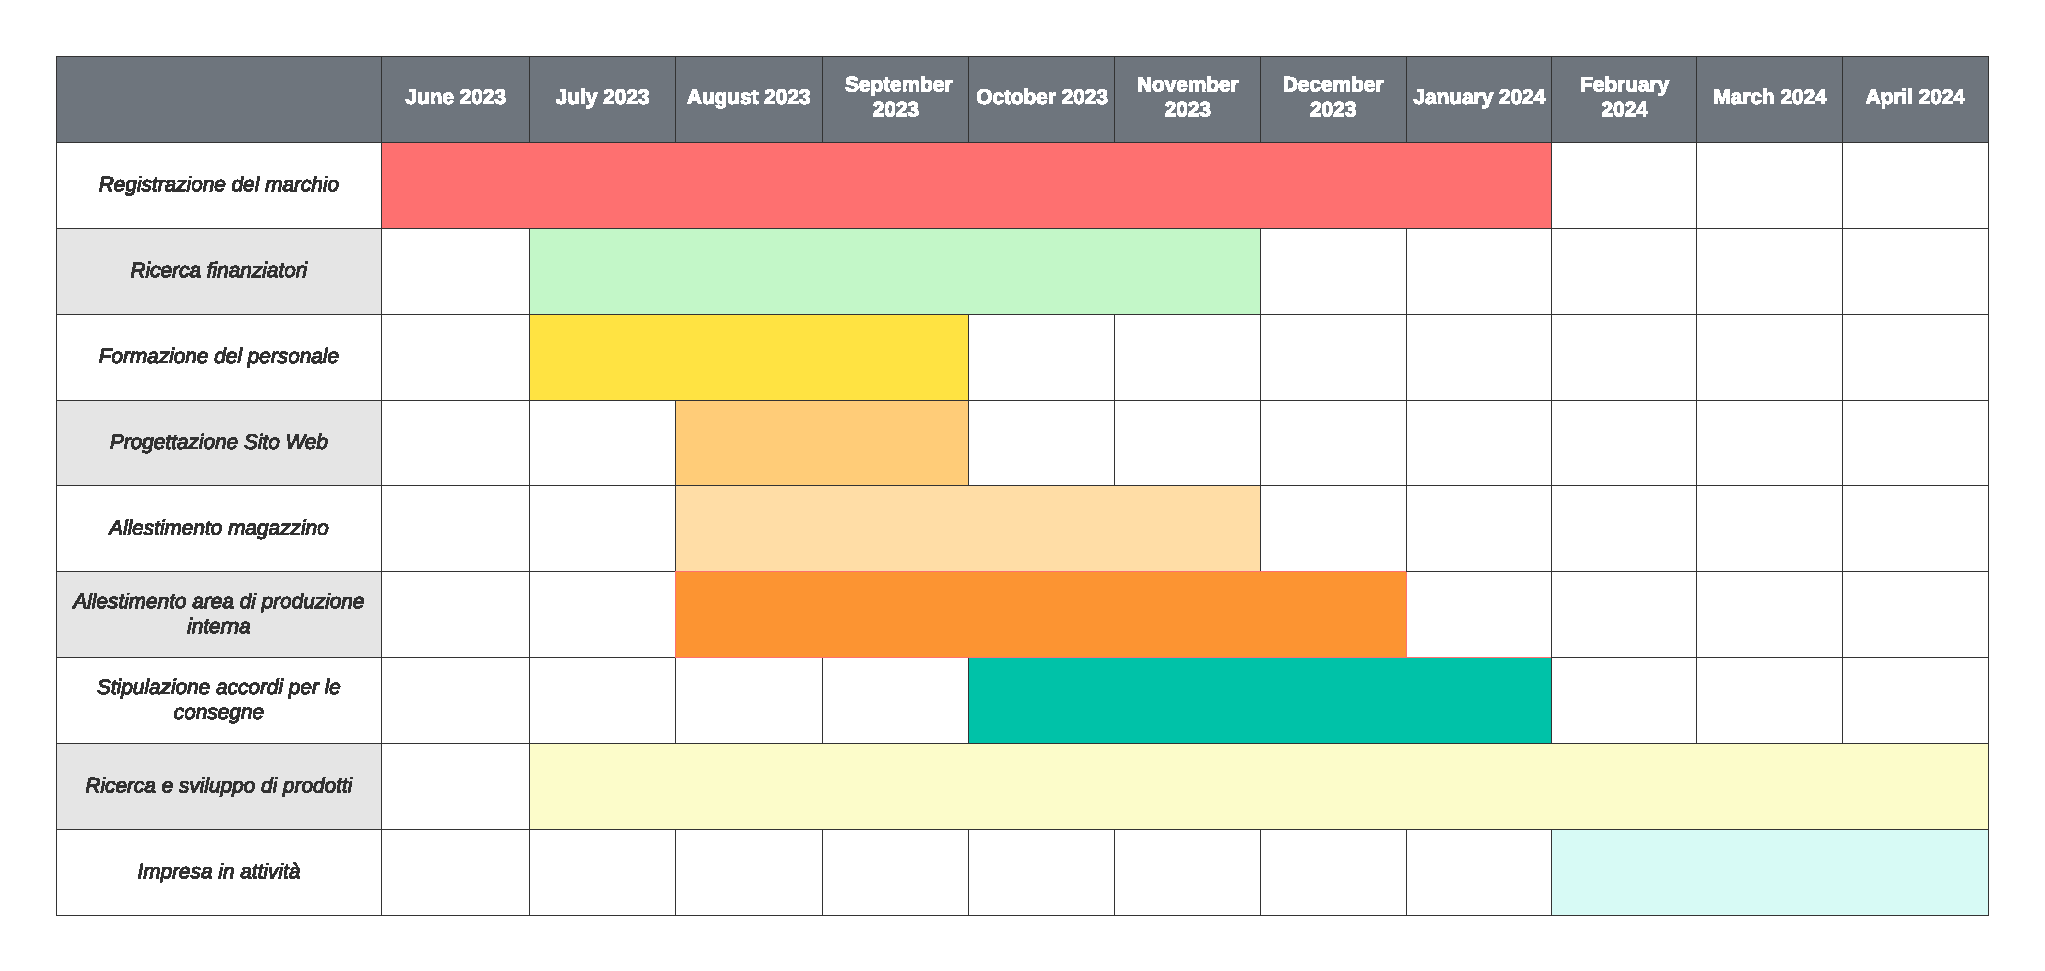
\includegraphics[width=\textwidth]{images/Diagramma_di_Gantt_di_base_1.pdf}

\section{Previsioni economico-finanziarie}
\begin{tabular}{|lccc|}
    \hline
    \rowcolor[HTML]{CBCEFB}
    \multicolumn{1}{|l|}{\cellcolor[HTML]{CBCEFB}}                                                                                   & \multicolumn{1}{c|}{\cellcolor[HTML]{CBCEFB}\textbf{1°esercizio}} & \multicolumn{1}{c|}{\cellcolor[HTML]{CBCEFB}\textbf{2°esercizio}} & \textbf{3°esercizio} \\ \hline
    \multicolumn{1}{|l|}{Ricavi di vendita}                                                                                          & \multicolumn{1}{c|}{278250,00}                                    & \multicolumn{1}{c|}{616.125,00}                                   & 1.371.375,00         \\ \hline
    \multicolumn{4}{|l|}{}                                                                                                                                                                                                                                                                          \\ \hline
    \multicolumn{1}{|l|}{Acquisto materie prime}                                                                                     & \multicolumn{1}{c|}{124075,00}                                    & \multicolumn{1}{c|}{274.737,50}                                   & 611.512,50           \\ \hline
    \multicolumn{1}{|l|}{Costi per servizi}                                                                                          & \multicolumn{1}{c|}{67025,00}                                     & \multicolumn{1}{c|}{148.412,50}                                   & 330.337,50           \\ \hline
    \multicolumn{1}{|l|}{Beni terzi}                                                                                                 & \multicolumn{1}{c|}{7.800,00}                                     & \multicolumn{1}{c|}{7.800,00}                                     & 7.800,00             \\ \hline
    \multicolumn{1}{|l|}{Variazione rimanenze}                                                                                       & \multicolumn{1}{c|}{- 2.280,00}                                   & \multicolumn{1}{c|}{- 1.725,00}                                   & - 7.302,50           \\ \hline
    \multicolumn{1}{|l|}{Costi industriali generali}                                                                                 & \multicolumn{1}{c|}{35.000,00}                                    & \multicolumn{1}{c|}{36530,00}                                     & 44880,00             \\ \hline
    \multicolumn{1}{|l|}{\cellcolor[HTML]{CBCEFB}\textbf{VALORE AGGIUNTO LORDO}}                                                     & \multicolumn{1}{c|}{46.630,00}                                    & \multicolumn{1}{c|}{150.370,00}                                   & 384.147,50           \\ \hline
    \multicolumn{4}{|l|}{}                                                                                                                                                                                                                                                                          \\ \hline
    \multicolumn{1}{|l|}{Costo del lavoro}                                                                                           & \multicolumn{1}{c|}{100.427,64}                                   & \multicolumn{1}{c|}{128.907,12}                                   & 206.850,96           \\ \hline
    \multicolumn{1}{|l|}{\cellcolor[HTML]{CBCEFB}\textbf{MARGINE OPERATIVO LORDO}}                                                   & \multicolumn{1}{c|}{-53797,64}                                    & \multicolumn{1}{c|}{21462,88}                                     & 177296,54            \\ \hline
    \multicolumn{4}{|l|}{}                                                                                                                                                                                                                                                                          \\ \hline
    \multicolumn{1}{|l|}{Ammortamenti}                                                                                               & \multicolumn{1}{c|}{17225,00}                                     & \multicolumn{1}{c|}{17225,00}                                     & 16725,00             \\ \hline
    \multicolumn{1}{|l|}{\cellcolor[HTML]{CBCEFB}\textbf{RISULTATO OPERATIVO GLOBALE}}                                               & \multicolumn{1}{c|}{-71022,64}                                    & \multicolumn{1}{c|}{4237,88}                                      & 160571,54            \\ \hline
    \multicolumn{4}{|l|}{}                                                                                                                                                                                                                                                                          \\ \hline
    \multicolumn{1}{|l|}{Oneri finanziari}                                                                                           & \multicolumn{1}{c|}{0,00}                                         & \multicolumn{1}{c|}{0,00}                                         & 0,00                 \\ \hline
    \multicolumn{1}{|l|}{\cellcolor[HTML]{CBCEFB}\textbf{RISULTATO ORDINARIO}}                                                       & \multicolumn{1}{c|}{-71022,64}                                    & \multicolumn{1}{c|}{4237,88}                                      & 160571,54            \\ \hline
    \multicolumn{4}{|l|}{}                                                                                                                                                                                                                                                                          \\ \hline
    \multicolumn{1}{|l|}{Proventi straordinari}                                                                                      & \multicolumn{1}{c|}{0,00}                                         & \multicolumn{1}{c|}{0,00}                                         & 0,00                 \\ \hline
    \multicolumn{1}{|l|}{Oneri straordinari}                                                                                         & \multicolumn{1}{c|}{0,00}                                         & \multicolumn{1}{c|}{0,00}                                         & 0,00                 \\ \hline
    \multicolumn{1}{|l|}{\cellcolor[HTML]{CBCEFB}\textbf{RISULTATO ANTE IMPOSTE}}                                                    & \multicolumn{1}{c|}{-71022,64}                                    & \multicolumn{1}{c|}{4237,88}                                      & 160571,54            \\ \hline
    \multicolumn{4}{|l|}{}                                                                                                                                                                                                                                                                          \\ \hline
    \multicolumn{1}{|l|}{Imposte sul reddito dell'esercizio}                                                                         & \multicolumn{1}{c|}{0,00}                                         & \multicolumn{1}{c|}{1082,86}                                      & 46372,73             \\ \hline
    \multicolumn{1}{|l|}{\cellcolor[HTML]{CBCEFB}\textbf{\begin{tabular}[c]{@{}l@{}}RISULTATO NETTO \\ DELL'ESERCIZIO\end{tabular}}} & \multicolumn{1}{c|}{-71022,64}                                    & \multicolumn{1}{c|}{3155,02}                                      & 114198,81            \\ \hline
\end{tabular}

\end{document}
